\documentclass[11pt]{article}

% Shared notes settings for Applied Machine Learning lectures (UPES).
% Keep this file free of \documentclass to allow reuse via \input.

\usepackage[utf8]{inputenc}
\usepackage[T1]{fontenc}
\usepackage{lmodern}          % scalable T1 fonts; without this pdflatex falls back
\input{glyphtounicode}        % to bitmapped EC Type 3 and the PDFs are neither
\pdfgentounicode=1            % searchable nor screen-reader friendly
\usepackage[a4paper,margin=1in]{geometry}
\usepackage{hyperref}
\usepackage{xurl}
\usepackage{booktabs}
\usepackage{amsmath}
\usepackage{amssymb}
\usepackage{listings}
\usepackage{xcolor}
\usepackage{enumitem}
\usepackage{parskip}

% Code listings (Python-oriented for this subject).
\lstset{
  language=Python,
  basicstyle=\ttfamily\small,
  keywordstyle=\color{blue},
  commentstyle=\color{gray},
  stringstyle=\color{teal},
  showstringspaces=false,
  columns=fullflexible,
  frame=single,
  framerule=0.2pt,
  breaklines=true
}

\setlist[itemize]{topsep=0.3em,itemsep=0.2em}
\setlist[enumerate]{topsep=0.3em,itemsep=0.2em}

% Simple per-section source line.
\newcommand{\notesources}[1]{\par\noindent{\small\color{gray}\textit{Sources:} \sloppy #1\par}}

% Unit-wise source strings for this subject (used by slides + notes).
% Path is relative to the lecture `latex/` folder (the compilation CWD).
\IfFileExists{../../../_shared/aml-sources.tex}{%
  % Source strings for Applied Machine Learning (CSAI2017P) — used by slides + notes.
% Prescribed texts and reference books are taken from the course syllabus.
% Support texts are the author-hosted open-access editions:
%   statlearning.com            (ISL with Python)
%   probml.github.io/pml-book   (Murphy, Probabilistic Machine Learning)
%   d2l.ai                      (Dive into Deep Learning)
%   mml-book.github.io          (Mathematics for Machine Learning)

\newcommand{\AMLRepoURL}{https://github.com/tali7c/Applied-Machine-Learning}

% --- prescribed -------------------------------------------------------------
\newcommand{\AMLPrescribed}{%
M\"uller and Guido, \textit{Introduction to Machine Learning with Python}, O'Reilly, 2016.;%
Bishop, \textit{Pattern Recognition and Machine Learning}, Springer, 2006.;%
Murphy, \textit{Machine Learning: A Probabilistic Perspective}, MIT Press, 2012.;%
Han, Kamber and Pei, \textit{Data Mining: Concepts and Techniques} (3e), Morgan Kaufmann, 2012.%
}

% --- unit-wise ---------------------------------------------------------------
\newcommand{\AMLUnitISources}{%
M\"uller and Guido, \textit{Introduction to Machine Learning with Python}, Ch. 1.;%
Bishop, \textit{Pattern Recognition and Machine Learning}, Ch. 1.;%
Murphy, \textit{Probabilistic Machine Learning: An Introduction}, MIT Press, 2022, Ch. 1.;%
Mitchell, \textit{Machine Learning}, McGraw Hill, 1997, Ch. 1.;%
Scikit-learn documentation, accessed 2026-08-04.%
}

\newcommand{\AMLUnitIISources}{%
Bishop, \textit{Pattern Recognition and Machine Learning}, \S1.5, \S4.3, \S7.1.;%
Zhang, Lipton, Li and Smola, \textit{Dive into Deep Learning}, \S3.4.;%
Shalev-Shwartz and Ben-David, \textit{Understanding Machine Learning}, Ch. 15.;%
Murphy, \textit{Probabilistic Machine Learning: An Introduction}, Ch. 5.%
}

\newcommand{\AMLUnitIIISources}{%
Zhang, Lipton, Li and Smola, \textit{Dive into Deep Learning}, Ch. 12 (Optimization Algorithms).;%
Deisenroth, Faisal and Ong, \textit{Mathematics for Machine Learning}, Ch. 7.;%
Kingma and Ba, ``Adam: A Method for Stochastic Optimization,'' ICLR 2015.;%
Ruder, ``An overview of gradient descent optimization algorithms,'' arXiv:1609.04747, 2016.%
}

\newcommand{\AMLUnitIVSources}{%
Han, Kamber and Pei, \textit{Data Mining: Concepts and Techniques} (3e), Ch. 3.;%
M\"uller and Guido, \textit{Introduction to Machine Learning with Python}, Ch. 3--4.;%
James, Witten, Hastie, Tibshirani and Taylor, \textit{An Introduction to Statistical Learning with Python}, Ch. 5--6, 12.;%
Scikit-learn documentation (preprocessing, model selection), accessed 2026-08-04.%
}

\newcommand{\AMLUnitVSources}{%
James et al., \textit{An Introduction to Statistical Learning with Python}, Ch. 3--6.;%
Bishop, \textit{Pattern Recognition and Machine Learning}, Ch. 3.;%
Deisenroth, Faisal and Ong, \textit{Mathematics for Machine Learning}, Ch. 9.;%
M\"uller and Guido, \textit{Introduction to Machine Learning with Python}, \S2.3.%
}

\newcommand{\AMLUnitVISources}{%
Han, Kamber and Pei, \textit{Data Mining: Concepts and Techniques} (3e), Ch. 8--9.;%
James et al., \textit{An Introduction to Statistical Learning with Python}, Ch. 8--9.;%
Bishop, \textit{Pattern Recognition and Machine Learning}, Ch. 4--5, 7, 14.;%
Zhang et al., \textit{Dive into Deep Learning}, Ch. 5.%
}

\newcommand{\AMLUnitVIISources}{%
Han, Kamber and Pei, \textit{Data Mining: Concepts and Techniques} (3e), Ch. 10.;%
James et al., \textit{An Introduction to Statistical Learning with Python}, Ch. 12.;%
M\"uller and Guido, \textit{Introduction to Machine Learning with Python}, \S3.5.;%
Ester, Kriegel, Sander and Xu, ``A density-based algorithm for discovering clusters (DBSCAN),'' KDD 1996.%
}

\newcommand{\AMLLabSources}{%
M\"uller and Guido, \textit{Introduction to Machine Learning with Python}, companion notebooks.;%
McKinney, \textit{Python for Data Analysis} (3e), O'Reilly, 2022.;%
Scikit-learn user guide, accessed 2026-08-04.;%
Matplotlib and Seaborn documentation, accessed 2026-08-04.%
}
%
}{%
  % Faculty copies live under `private/` so their compile CWD is different.
  \IfFileExists{../../../../public/_shared/aml-sources.tex}{%
    % Source strings for Applied Machine Learning (CSAI2017P) — used by slides + notes.
% Prescribed texts and reference books are taken from the course syllabus.
% Support texts are the author-hosted open-access editions:
%   statlearning.com            (ISL with Python)
%   probml.github.io/pml-book   (Murphy, Probabilistic Machine Learning)
%   d2l.ai                      (Dive into Deep Learning)
%   mml-book.github.io          (Mathematics for Machine Learning)

\newcommand{\AMLRepoURL}{https://github.com/tali7c/Applied-Machine-Learning}

% --- prescribed -------------------------------------------------------------
\newcommand{\AMLPrescribed}{%
M\"uller and Guido, \textit{Introduction to Machine Learning with Python}, O'Reilly, 2016.;%
Bishop, \textit{Pattern Recognition and Machine Learning}, Springer, 2006.;%
Murphy, \textit{Machine Learning: A Probabilistic Perspective}, MIT Press, 2012.;%
Han, Kamber and Pei, \textit{Data Mining: Concepts and Techniques} (3e), Morgan Kaufmann, 2012.%
}

% --- unit-wise ---------------------------------------------------------------
\newcommand{\AMLUnitISources}{%
M\"uller and Guido, \textit{Introduction to Machine Learning with Python}, Ch. 1.;%
Bishop, \textit{Pattern Recognition and Machine Learning}, Ch. 1.;%
Murphy, \textit{Probabilistic Machine Learning: An Introduction}, MIT Press, 2022, Ch. 1.;%
Mitchell, \textit{Machine Learning}, McGraw Hill, 1997, Ch. 1.;%
Scikit-learn documentation, accessed 2026-08-04.%
}

\newcommand{\AMLUnitIISources}{%
Bishop, \textit{Pattern Recognition and Machine Learning}, \S1.5, \S4.3, \S7.1.;%
Zhang, Lipton, Li and Smola, \textit{Dive into Deep Learning}, \S3.4.;%
Shalev-Shwartz and Ben-David, \textit{Understanding Machine Learning}, Ch. 15.;%
Murphy, \textit{Probabilistic Machine Learning: An Introduction}, Ch. 5.%
}

\newcommand{\AMLUnitIIISources}{%
Zhang, Lipton, Li and Smola, \textit{Dive into Deep Learning}, Ch. 12 (Optimization Algorithms).;%
Deisenroth, Faisal and Ong, \textit{Mathematics for Machine Learning}, Ch. 7.;%
Kingma and Ba, ``Adam: A Method for Stochastic Optimization,'' ICLR 2015.;%
Ruder, ``An overview of gradient descent optimization algorithms,'' arXiv:1609.04747, 2016.%
}

\newcommand{\AMLUnitIVSources}{%
Han, Kamber and Pei, \textit{Data Mining: Concepts and Techniques} (3e), Ch. 3.;%
M\"uller and Guido, \textit{Introduction to Machine Learning with Python}, Ch. 3--4.;%
James, Witten, Hastie, Tibshirani and Taylor, \textit{An Introduction to Statistical Learning with Python}, Ch. 5--6, 12.;%
Scikit-learn documentation (preprocessing, model selection), accessed 2026-08-04.%
}

\newcommand{\AMLUnitVSources}{%
James et al., \textit{An Introduction to Statistical Learning with Python}, Ch. 3--6.;%
Bishop, \textit{Pattern Recognition and Machine Learning}, Ch. 3.;%
Deisenroth, Faisal and Ong, \textit{Mathematics for Machine Learning}, Ch. 9.;%
M\"uller and Guido, \textit{Introduction to Machine Learning with Python}, \S2.3.%
}

\newcommand{\AMLUnitVISources}{%
Han, Kamber and Pei, \textit{Data Mining: Concepts and Techniques} (3e), Ch. 8--9.;%
James et al., \textit{An Introduction to Statistical Learning with Python}, Ch. 8--9.;%
Bishop, \textit{Pattern Recognition and Machine Learning}, Ch. 4--5, 7, 14.;%
Zhang et al., \textit{Dive into Deep Learning}, Ch. 5.%
}

\newcommand{\AMLUnitVIISources}{%
Han, Kamber and Pei, \textit{Data Mining: Concepts and Techniques} (3e), Ch. 10.;%
James et al., \textit{An Introduction to Statistical Learning with Python}, Ch. 12.;%
M\"uller and Guido, \textit{Introduction to Machine Learning with Python}, \S3.5.;%
Ester, Kriegel, Sander and Xu, ``A density-based algorithm for discovering clusters (DBSCAN),'' KDD 1996.%
}

\newcommand{\AMLLabSources}{%
M\"uller and Guido, \textit{Introduction to Machine Learning with Python}, companion notebooks.;%
McKinney, \textit{Python for Data Analysis} (3e), O'Reilly, 2022.;%
Scikit-learn user guide, accessed 2026-08-04.;%
Matplotlib and Seaborn documentation, accessed 2026-08-04.%
}
%
  }{%
    % Question papers live at `private/<family>/<instrument>/`.
    \IfFileExists{../../../public/_shared/aml-sources.tex}{%
      % Source strings for Applied Machine Learning (CSAI2017P) — used by slides + notes.
% Prescribed texts and reference books are taken from the course syllabus.
% Support texts are the author-hosted open-access editions:
%   statlearning.com            (ISL with Python)
%   probml.github.io/pml-book   (Murphy, Probabilistic Machine Learning)
%   d2l.ai                      (Dive into Deep Learning)
%   mml-book.github.io          (Mathematics for Machine Learning)

\newcommand{\AMLRepoURL}{https://github.com/tali7c/Applied-Machine-Learning}

% --- prescribed -------------------------------------------------------------
\newcommand{\AMLPrescribed}{%
M\"uller and Guido, \textit{Introduction to Machine Learning with Python}, O'Reilly, 2016.;%
Bishop, \textit{Pattern Recognition and Machine Learning}, Springer, 2006.;%
Murphy, \textit{Machine Learning: A Probabilistic Perspective}, MIT Press, 2012.;%
Han, Kamber and Pei, \textit{Data Mining: Concepts and Techniques} (3e), Morgan Kaufmann, 2012.%
}

% --- unit-wise ---------------------------------------------------------------
\newcommand{\AMLUnitISources}{%
M\"uller and Guido, \textit{Introduction to Machine Learning with Python}, Ch. 1.;%
Bishop, \textit{Pattern Recognition and Machine Learning}, Ch. 1.;%
Murphy, \textit{Probabilistic Machine Learning: An Introduction}, MIT Press, 2022, Ch. 1.;%
Mitchell, \textit{Machine Learning}, McGraw Hill, 1997, Ch. 1.;%
Scikit-learn documentation, accessed 2026-08-04.%
}

\newcommand{\AMLUnitIISources}{%
Bishop, \textit{Pattern Recognition and Machine Learning}, \S1.5, \S4.3, \S7.1.;%
Zhang, Lipton, Li and Smola, \textit{Dive into Deep Learning}, \S3.4.;%
Shalev-Shwartz and Ben-David, \textit{Understanding Machine Learning}, Ch. 15.;%
Murphy, \textit{Probabilistic Machine Learning: An Introduction}, Ch. 5.%
}

\newcommand{\AMLUnitIIISources}{%
Zhang, Lipton, Li and Smola, \textit{Dive into Deep Learning}, Ch. 12 (Optimization Algorithms).;%
Deisenroth, Faisal and Ong, \textit{Mathematics for Machine Learning}, Ch. 7.;%
Kingma and Ba, ``Adam: A Method for Stochastic Optimization,'' ICLR 2015.;%
Ruder, ``An overview of gradient descent optimization algorithms,'' arXiv:1609.04747, 2016.%
}

\newcommand{\AMLUnitIVSources}{%
Han, Kamber and Pei, \textit{Data Mining: Concepts and Techniques} (3e), Ch. 3.;%
M\"uller and Guido, \textit{Introduction to Machine Learning with Python}, Ch. 3--4.;%
James, Witten, Hastie, Tibshirani and Taylor, \textit{An Introduction to Statistical Learning with Python}, Ch. 5--6, 12.;%
Scikit-learn documentation (preprocessing, model selection), accessed 2026-08-04.%
}

\newcommand{\AMLUnitVSources}{%
James et al., \textit{An Introduction to Statistical Learning with Python}, Ch. 3--6.;%
Bishop, \textit{Pattern Recognition and Machine Learning}, Ch. 3.;%
Deisenroth, Faisal and Ong, \textit{Mathematics for Machine Learning}, Ch. 9.;%
M\"uller and Guido, \textit{Introduction to Machine Learning with Python}, \S2.3.%
}

\newcommand{\AMLUnitVISources}{%
Han, Kamber and Pei, \textit{Data Mining: Concepts and Techniques} (3e), Ch. 8--9.;%
James et al., \textit{An Introduction to Statistical Learning with Python}, Ch. 8--9.;%
Bishop, \textit{Pattern Recognition and Machine Learning}, Ch. 4--5, 7, 14.;%
Zhang et al., \textit{Dive into Deep Learning}, Ch. 5.%
}

\newcommand{\AMLUnitVIISources}{%
Han, Kamber and Pei, \textit{Data Mining: Concepts and Techniques} (3e), Ch. 10.;%
James et al., \textit{An Introduction to Statistical Learning with Python}, Ch. 12.;%
M\"uller and Guido, \textit{Introduction to Machine Learning with Python}, \S3.5.;%
Ester, Kriegel, Sander and Xu, ``A density-based algorithm for discovering clusters (DBSCAN),'' KDD 1996.%
}

\newcommand{\AMLLabSources}{%
M\"uller and Guido, \textit{Introduction to Machine Learning with Python}, companion notebooks.;%
McKinney, \textit{Python for Data Analysis} (3e), O'Reilly, 2022.;%
Scikit-learn user guide, accessed 2026-08-04.;%
Matplotlib and Seaborn documentation, accessed 2026-08-04.%
}
%
    }{%
      % Marking schemes live at `private/solutions/<family>/<id>/latex/`.
      \IfFileExists{../../../../../public/_shared/aml-sources.tex}{%
        % Source strings for Applied Machine Learning (CSAI2017P) — used by slides + notes.
% Prescribed texts and reference books are taken from the course syllabus.
% Support texts are the author-hosted open-access editions:
%   statlearning.com            (ISL with Python)
%   probml.github.io/pml-book   (Murphy, Probabilistic Machine Learning)
%   d2l.ai                      (Dive into Deep Learning)
%   mml-book.github.io          (Mathematics for Machine Learning)

\newcommand{\AMLRepoURL}{https://github.com/tali7c/Applied-Machine-Learning}

% --- prescribed -------------------------------------------------------------
\newcommand{\AMLPrescribed}{%
M\"uller and Guido, \textit{Introduction to Machine Learning with Python}, O'Reilly, 2016.;%
Bishop, \textit{Pattern Recognition and Machine Learning}, Springer, 2006.;%
Murphy, \textit{Machine Learning: A Probabilistic Perspective}, MIT Press, 2012.;%
Han, Kamber and Pei, \textit{Data Mining: Concepts and Techniques} (3e), Morgan Kaufmann, 2012.%
}

% --- unit-wise ---------------------------------------------------------------
\newcommand{\AMLUnitISources}{%
M\"uller and Guido, \textit{Introduction to Machine Learning with Python}, Ch. 1.;%
Bishop, \textit{Pattern Recognition and Machine Learning}, Ch. 1.;%
Murphy, \textit{Probabilistic Machine Learning: An Introduction}, MIT Press, 2022, Ch. 1.;%
Mitchell, \textit{Machine Learning}, McGraw Hill, 1997, Ch. 1.;%
Scikit-learn documentation, accessed 2026-08-04.%
}

\newcommand{\AMLUnitIISources}{%
Bishop, \textit{Pattern Recognition and Machine Learning}, \S1.5, \S4.3, \S7.1.;%
Zhang, Lipton, Li and Smola, \textit{Dive into Deep Learning}, \S3.4.;%
Shalev-Shwartz and Ben-David, \textit{Understanding Machine Learning}, Ch. 15.;%
Murphy, \textit{Probabilistic Machine Learning: An Introduction}, Ch. 5.%
}

\newcommand{\AMLUnitIIISources}{%
Zhang, Lipton, Li and Smola, \textit{Dive into Deep Learning}, Ch. 12 (Optimization Algorithms).;%
Deisenroth, Faisal and Ong, \textit{Mathematics for Machine Learning}, Ch. 7.;%
Kingma and Ba, ``Adam: A Method for Stochastic Optimization,'' ICLR 2015.;%
Ruder, ``An overview of gradient descent optimization algorithms,'' arXiv:1609.04747, 2016.%
}

\newcommand{\AMLUnitIVSources}{%
Han, Kamber and Pei, \textit{Data Mining: Concepts and Techniques} (3e), Ch. 3.;%
M\"uller and Guido, \textit{Introduction to Machine Learning with Python}, Ch. 3--4.;%
James, Witten, Hastie, Tibshirani and Taylor, \textit{An Introduction to Statistical Learning with Python}, Ch. 5--6, 12.;%
Scikit-learn documentation (preprocessing, model selection), accessed 2026-08-04.%
}

\newcommand{\AMLUnitVSources}{%
James et al., \textit{An Introduction to Statistical Learning with Python}, Ch. 3--6.;%
Bishop, \textit{Pattern Recognition and Machine Learning}, Ch. 3.;%
Deisenroth, Faisal and Ong, \textit{Mathematics for Machine Learning}, Ch. 9.;%
M\"uller and Guido, \textit{Introduction to Machine Learning with Python}, \S2.3.%
}

\newcommand{\AMLUnitVISources}{%
Han, Kamber and Pei, \textit{Data Mining: Concepts and Techniques} (3e), Ch. 8--9.;%
James et al., \textit{An Introduction to Statistical Learning with Python}, Ch. 8--9.;%
Bishop, \textit{Pattern Recognition and Machine Learning}, Ch. 4--5, 7, 14.;%
Zhang et al., \textit{Dive into Deep Learning}, Ch. 5.%
}

\newcommand{\AMLUnitVIISources}{%
Han, Kamber and Pei, \textit{Data Mining: Concepts and Techniques} (3e), Ch. 10.;%
James et al., \textit{An Introduction to Statistical Learning with Python}, Ch. 12.;%
M\"uller and Guido, \textit{Introduction to Machine Learning with Python}, \S3.5.;%
Ester, Kriegel, Sander and Xu, ``A density-based algorithm for discovering clusters (DBSCAN),'' KDD 1996.%
}

\newcommand{\AMLLabSources}{%
M\"uller and Guido, \textit{Introduction to Machine Learning with Python}, companion notebooks.;%
McKinney, \textit{Python for Data Analysis} (3e), O'Reilly, 2022.;%
Scikit-learn user guide, accessed 2026-08-04.;%
Matplotlib and Seaborn documentation, accessed 2026-08-04.%
}
%
      }{%
        % Source strings for Applied Machine Learning (CSAI2017P) — used by slides + notes.
% Prescribed texts and reference books are taken from the course syllabus.
% Support texts are the author-hosted open-access editions:
%   statlearning.com            (ISL with Python)
%   probml.github.io/pml-book   (Murphy, Probabilistic Machine Learning)
%   d2l.ai                      (Dive into Deep Learning)
%   mml-book.github.io          (Mathematics for Machine Learning)

\newcommand{\AMLRepoURL}{https://github.com/tali7c/Applied-Machine-Learning}

% --- prescribed -------------------------------------------------------------
\newcommand{\AMLPrescribed}{%
M\"uller and Guido, \textit{Introduction to Machine Learning with Python}, O'Reilly, 2016.;%
Bishop, \textit{Pattern Recognition and Machine Learning}, Springer, 2006.;%
Murphy, \textit{Machine Learning: A Probabilistic Perspective}, MIT Press, 2012.;%
Han, Kamber and Pei, \textit{Data Mining: Concepts and Techniques} (3e), Morgan Kaufmann, 2012.%
}

% --- unit-wise ---------------------------------------------------------------
\newcommand{\AMLUnitISources}{%
M\"uller and Guido, \textit{Introduction to Machine Learning with Python}, Ch. 1.;%
Bishop, \textit{Pattern Recognition and Machine Learning}, Ch. 1.;%
Murphy, \textit{Probabilistic Machine Learning: An Introduction}, MIT Press, 2022, Ch. 1.;%
Mitchell, \textit{Machine Learning}, McGraw Hill, 1997, Ch. 1.;%
Scikit-learn documentation, accessed 2026-08-04.%
}

\newcommand{\AMLUnitIISources}{%
Bishop, \textit{Pattern Recognition and Machine Learning}, \S1.5, \S4.3, \S7.1.;%
Zhang, Lipton, Li and Smola, \textit{Dive into Deep Learning}, \S3.4.;%
Shalev-Shwartz and Ben-David, \textit{Understanding Machine Learning}, Ch. 15.;%
Murphy, \textit{Probabilistic Machine Learning: An Introduction}, Ch. 5.%
}

\newcommand{\AMLUnitIIISources}{%
Zhang, Lipton, Li and Smola, \textit{Dive into Deep Learning}, Ch. 12 (Optimization Algorithms).;%
Deisenroth, Faisal and Ong, \textit{Mathematics for Machine Learning}, Ch. 7.;%
Kingma and Ba, ``Adam: A Method for Stochastic Optimization,'' ICLR 2015.;%
Ruder, ``An overview of gradient descent optimization algorithms,'' arXiv:1609.04747, 2016.%
}

\newcommand{\AMLUnitIVSources}{%
Han, Kamber and Pei, \textit{Data Mining: Concepts and Techniques} (3e), Ch. 3.;%
M\"uller and Guido, \textit{Introduction to Machine Learning with Python}, Ch. 3--4.;%
James, Witten, Hastie, Tibshirani and Taylor, \textit{An Introduction to Statistical Learning with Python}, Ch. 5--6, 12.;%
Scikit-learn documentation (preprocessing, model selection), accessed 2026-08-04.%
}

\newcommand{\AMLUnitVSources}{%
James et al., \textit{An Introduction to Statistical Learning with Python}, Ch. 3--6.;%
Bishop, \textit{Pattern Recognition and Machine Learning}, Ch. 3.;%
Deisenroth, Faisal and Ong, \textit{Mathematics for Machine Learning}, Ch. 9.;%
M\"uller and Guido, \textit{Introduction to Machine Learning with Python}, \S2.3.%
}

\newcommand{\AMLUnitVISources}{%
Han, Kamber and Pei, \textit{Data Mining: Concepts and Techniques} (3e), Ch. 8--9.;%
James et al., \textit{An Introduction to Statistical Learning with Python}, Ch. 8--9.;%
Bishop, \textit{Pattern Recognition and Machine Learning}, Ch. 4--5, 7, 14.;%
Zhang et al., \textit{Dive into Deep Learning}, Ch. 5.%
}

\newcommand{\AMLUnitVIISources}{%
Han, Kamber and Pei, \textit{Data Mining: Concepts and Techniques} (3e), Ch. 10.;%
James et al., \textit{An Introduction to Statistical Learning with Python}, Ch. 12.;%
M\"uller and Guido, \textit{Introduction to Machine Learning with Python}, \S3.5.;%
Ester, Kriegel, Sander and Xu, ``A density-based algorithm for discovering clusters (DBSCAN),'' KDD 1996.%
}

\newcommand{\AMLLabSources}{%
M\"uller and Guido, \textit{Introduction to Machine Learning with Python}, companion notebooks.;%
McKinney, \textit{Python for Data Analysis} (3e), O'Reilly, 2022.;%
Scikit-learn user guide, accessed 2026-08-04.;%
Matplotlib and Seaborn documentation, accessed 2026-08-04.%
}
%
      }%
    }%
  }%
}


\graphicspath{{../figures/}}

% This lecture pairs almost every paragraph with a listing and its output, so
% the default \medskipamount around each block adds up to several pages.
\lstset{aboveskip=3pt, belowskip=3pt}
\lstdefinestyle{amlout}{language={}, keepspaces=true,
  basicstyle=\ttfamily\footnotesize\color{black!80},
  backgroundcolor=\color{black!4}, frame=leftline, framerule=2pt,
  rulecolor=\color{black!25}, breaklines=true, columns=fullflexible,
  xleftmargin=8pt, aboveskip=2pt, belowskip=4pt, literate={-}{{-}}1}
\captionsetup{skip=4pt, font=small}
% Ten wide figures in a text-dense document: let them share pages with prose
% instead of being pushed onto float pages of their own.
\renewcommand{\topfraction}{0.92}
\renewcommand{\bottomfraction}{0.75}
\renewcommand{\textfraction}{0.06}
\renewcommand{\floatpagefraction}{0.85}
\setlength{\floatsep}{6pt plus 2pt minus 2pt}
\setlength{\textfloatsep}{8pt plus 2pt minus 2pt}
\setlength{\intextsep}{8pt plus 2pt minus 2pt}

\title{Applied Machine Learning\\Unit 04 --- Lecture 06 Notes\\
       Feature Engineering, Encoding and Dimensionality Reduction}
\author{Tofik Ali}
\date{Autumn 2026}

\begin{document}
\maketitle

\begin{keyidea}[Read this first]
These notes are written so that you can learn the material \emph{without}
having been in the lecture. Every concept is developed from scratch, every
number you see was produced by running the code shown beside it, and every
figure was generated from real computation rather than drawn by hand.

The previous lecture cleaned the table: holes filled, stuck sensors found,
long tails straightened. It ended on one rule --- \emph{every number used to
clean the data must be computed from the training rows only}. The table is now
clean. It is not yet usable. The columns are in different units, some of them
are words rather than numbers, and there may be far more of them than the
problem needs.

Four questions organise this lecture. What should the columns \textbf{be}?
What \textbf{units} should they be in? What do I do with a column of
\textbf{words}? And what do I do when there are \textbf{too many columns}?

The single result to carry out of the lecture: a logistic regression scored
$\mathbf{0.8475}$ on a table of $500$ pure-noise features and $60$ rows whose
labels were coin flips. The only thing wrong with the experiment was that the
features were chosen before the data was split. Work through
Section~\ref{sec:selectleak} with a Python session open until you can say
exactly why.
\end{keyidea}

\tableofcontents
\medskip

% =========================================================================
\section{How to use these notes}
\label{sec:how}

Read in order. Section~\ref{sec:pca} assumes the scaling material of
Section~\ref{sec:scale}, and Section~\ref{sec:select} contrasts itself
throughout with Section~\ref{sec:pca}. Everything here assumes only what
Lecture~5 assumed: a train/test split, a fitted model and a score. The one new
piece of mathematics is the eigen-decomposition of a $2\times2$ symmetric
matrix, done by hand in Section~\ref{sec:pcahand}.

There are four kinds of box. \textbf{Key idea} --- the one sentence to
remember a month from now. \textbf{Worked example} --- a calculation done by
hand, with small numbers, before any library is used. \textbf{Caution} --- the
specific mistake that section exists to prevent. \textbf{Try it yourself} ---
something to run, with the expected output given so you can check.

Code appears in a framed block, and directly beneath it a shaded block showing
what that code \emph{actually printed}. If you run it and get something
different, trust your machine and tell me.

\subsection{What you need}

\begin{lstlisting}
pip install numpy scipy scikit-learn matplotlib pandas
\end{lstlisting}

Every number in these notes was produced with:

\begin{lstlisting}
import numpy, scipy, sklearn, matplotlib
print("numpy", numpy.__version__, "| scipy", scipy.__version__,
      "| sklearn", sklearn.__version__,
      "| matplotlib", matplotlib.__version__)
\end{lstlisting}
\begin{codeout}
numpy 2.2.6 | scipy 1.15.3 | sklearn 1.7.2 | matplotlib 3.10.9
\end{codeout}

Four bundled datasets recur, and \textbf{none of them downloads anything}.

\begin{lstlisting}
from sklearn.datasets import (load_breast_cancer, load_digits,
                              load_wine, load_diabetes)
bc = load_breast_cancer();  Xb, yb = bc.data, bc.target
dg = load_digits();         Xg, yg = dg.data, dg.target
wine = load_wine();         Xw, yw = wine.data, wine.target
dia = load_diabetes();      Xd, yd = dia.data, dia.target.astype(float)
\end{lstlisting}
\begin{codeout}
load_breast_cancer 569 rows x 30 features, 2 classes
load_digits        1797 rows x 64 features, 10 classes
load_wine          178 rows x 13 features, 3 classes
load_diabetes      442 rows x 10 features, continuous target
missing cells anywhere: 0
feature scales in breast_cancer differ by a factor of 215171
\end{codeout}

That last line is why \texttt{load\_breast\_cancer} is the running example:
its widest column has a standard deviation two hundred thousand times the
narrowest, which is exactly the situation this lecture is about.

\begin{keyidea}[Four datasets, one seed --- the convention for this lecture]
Everything in these notes is computed from the four bundled tables above,
plus a handful of small problems drawn on the spot to make a specific point,
and \textbf{one seed}. The seed is \textbf{0}: every generator is created as
\texttt{np.random.default\_rng(0)}, every stochastic estimator is given
\texttt{random\_state=0} --- including \texttt{mutual\_info\_classif},
which is stochastic and silently gives you a different answer without one ---
and the cross-validation shuffle is \texttt{StratifiedKFold(5, shuffle=True,
random\_state=0)}. Every listing below that involves chance shows that line.

The exceptions are the two \emph{sweeps}: the forty train/test splits of
Section~\ref{sec:pcaleak} and the twenty repetitions of
Section~\ref{sec:selectleak} use a
different seed each time, on purpose, because the variation between
repetitions is the thing being measured. Their seeds are still derived from
the same $0$, so the sweep as a whole reproduces exactly.

Run the code as written and you get the numbers printed here. If you get
something different, the difference is in your code or your library versions,
not in chance.
\end{keyidea}

\begin{caution}[Do not reach for \texttt{fetch\_*}]
Every \texttt{fetch\_*} loader downloads over HTTPS, and on the campus network
those downloads fail with a certificate error you cannot fix from your machine.
Nothing in this course depends on one: use the bundled loaders
(\texttt{load\_diabetes}, \texttt{load\_breast\_cancer}, \texttt{load\_iris},
\texttt{load\_wine}, \texttt{load\_digits}) or a fixed-seed synthetic set.
\end{caution}

\subsection{Learning outcomes}

By the end of this lecture you should be able to:

\begin{enumerate}[leftmargin=*]
  \item Construct new features by combining, decomposing, binning and
    transforming existing ones, and say which models such engineering helps
    and which it does not (CO2).
  \item Apply standardisation, min--max, robust and max-abs scaling; derive
    each from its formula on a small vector by hand; and predict which
    learning algorithms change their answer when the data is rescaled and
    which cannot (CO2).
  \item Encode nominal and ordinal categorical variables correctly, explain
    and avoid the dummy variable trap, and quantify the cost of one-hot
    encoding a high-cardinality column (CO2).
  \item State Han, Kamber and Pei's three kinds of data reduction ---
    dimensionality, numerosity and compression --- and give a worked example
    of each (CO2).
  \item Compute a principal component analysis by hand on a small dataset,
    interpret the variance-explained curve, choose $k$, quantify
    reconstruction error, and explain why PCA must be fitted on the training
    split and preceded by scaling (CO2).
  \item Distinguish filter, wrapper and embedded feature selection; apply
    variance thresholds, ANOVA $F$, mutual information, recursive feature
    elimination and L1 regularisation; and identify selection bias in a
    described workflow (CO2).
\end{enumerate}

% =========================================================================
\section{Feature engineering}
\label{sec:fe}

\subsection{What it is, and why it is worth more than the algorithm}

\textbf{Feature engineering} is choosing the representation of the data that
the model sees. It is the least glamorous and most consequential thing in the
subject, and Müller and Guido open their chapter on it with the claim that
\emph{how you represent your data matters more than which algorithm you pick}.

Four moves cover almost everything you will do.

\begin{enumerate}[leftmargin=*]
  \item \textbf{Combine.} Length and width become area. Height and weight
    become body mass index. Two timestamps become a duration.
  \item \textbf{Decompose.} A timestamp becomes hour-of-day, day-of-week and
    month. An address becomes a postcode and a city.
  \item \textbf{Bin.} A continuous variable becomes a set of intervals, so a
    linear model can fit a step function.
  \item \textbf{Transform.} $\log$, square root, ratios, differences. This is
    the Lecture~5 material seen from the other side.
\end{enumerate}

\begin{keyidea}
A linear model can only add its inputs up. If the quantity that matters is a
product, a ratio or a threshold, no amount of optimisation will find it --- but
one new column will.
\end{keyidea}

\subsection{Worked: four plots of land}
\label{sec:land}

\begin{worked}[The information is there; the representation is hiding it]
Four rectangular plots. The price is $5$ per square metre, in rupees. Nobody
recorded the area.
\begin{center}
\begin{tabular}{@{}lrrrr@{}}
\toprule
length $\ell$ (m) & $10$ & $20$ & $30$ & $40$\\
width $w$ (m)     & $40$ & $15$ & $20$ & $12$\\
\midrule
area $= \ell w$   & $400$ & $300$ & $600$ & $480$\\
price $= 5\ell w$ & $2000$ & $1500$ & $3000$ & $2400$\\
\bottomrule
\end{tabular}
\end{center}
The price is a perfect deterministic function of the two recorded columns, but
it is not a \emph{linear} one, and the correlations show it:
\[
  \mathrm{corr}(\text{price}, \ell) = +0.5494, \qquad
  \mathrm{corr}(\text{price}, w) = -0.0948, \qquad
  \mathrm{corr}(\text{price}, \ell w) = +1.0000 .
\]
The width even appears \emph{negatively} associated with price, which is an
artefact of the four plots we happen to have. A linear model on $(\ell, w)$
reaches $R^2 = 0.6558$; add the column $\ell w$ and it reaches $1.0000$.
\end{worked}

\begin{lstlisting}
length = np.array([10., 20., 30., 40.])
width  = np.array([40., 15., 20., 12.])
price  = 5.0 * length * width
LinearRegression().fit(np.c_[length, width], price).score(...)
LinearRegression().fit(np.c_[length, width, length * width], price).score(...)
\end{lstlisting}
\begin{codeout}
corr(price, length) = +0.5494
corr(price, width ) = -0.0948
corr(price, area  ) = +1.0000
R2 of a linear model on (length, width)       0.6558
R2 of a linear model on (length, width, area) 1.0000
\end{codeout}

Four rows is too few to be convincing. Here is the same idea on $400$ rows with
noise, cross-validated.

\begin{lstlisting}
rng = np.random.default_rng(0)               # the one seed for this lecture
x1, x2 = rng.uniform(1, 10, 400), rng.uniform(1, 10, 400)
y = 3.0 * x1 * x2 + rng.normal(0, 3.0, 400)
for X in (np.c_[x1, x2], np.c_[x1, x2, x1 * x2]):
    print(cross_val_score(LinearRegression(), X, y, cv=5, scoring="r2").mean())
\end{lstlisting}
\begin{codeout}
linear model on x1, x2          cross-validated R2 0.9091
linear model on x1, x2, x1*x2   cross-validated R2 0.9981
a random forest on the raw pair gets there too, accuracy 0.9650
\end{codeout}

Read the third line as carefully as the first two. A tree finds an interaction
unaided, by splitting twice; the engineered column is worth a great deal to a
linear model and almost nothing to a forest. \textbf{Feature engineering is
worth most to the simplest models}, which is one reason simple models plus
good features remain competitive.

\subsection{Binning, and why a representation is only good relative to a model}
\label{sec:binning}

\texttt{KBinsDiscretizer} cuts a continuous column into intervals and one-hot
encodes the interval. A linear model on those indicator columns is a step
function, so binning buys a linear model the flexibility it did not have.

\begin{lstlisting}
kb = KBinsDiscretizer(n_bins=10, encode="onehot-dense", strategy="uniform")
cross_val_score(make_pipeline(kb, LinearRegression()), x, y, cv=5, scoring="r2")
\end{lstlisting}
\begin{codeout}
one wiggly feature, 250 points, y = sin(4x) + x + noise
                            raw x    10 bins
LinearRegression           0.8194     0.9151
DecisionTreeRegressor      0.9475     0.9151
binning bought the linear model +0.0957 and cost the tree -0.0323
\end{codeout}

The two scores after binning are \emph{identical to four decimal places}, and
that is not a coincidence: after binning, both models are fitting a step
function on the same ten intervals, so they are fitting the same family. The
tree lost $0.0323$ because it had been choosing its own cut points and we took
that away.

\begin{keyidea}
A representation is not good or bad in the abstract. It is good or bad
\emph{relative to a model}. Binning helps linear models and hurts trees.
\end{keyidea}

\subsection{Engineering blind: the combinatorial blow-up}
\label{sec:poly}

If products help, why not add all of them? \texttt{PolynomialFeatures(degree=k)}
does exactly that, and the count is $\binom{d+k}{k}-1$, which grows like $d^k$.

\begin{codeout}
  d=2   degree 2 ->     5 features  d=2   degree 3 ->     9 features
  d=10  degree 2 ->    65 features  d=10  degree 3 ->   285 features
  d=30  degree 2 ->   495 features  d=30  degree 3 ->  5455 features
  d=64  degree 2 ->  2144 features  d=64  degree 3 -> 47904 features
\end{codeout}

\begin{lstlisting}
X2 = PolynomialFeatures(degree=2, include_bias=False).fit_transform(Xd)
cross_val_score(make_pipeline(StandardScaler(), Ridge(1.0)), X2, yd,
                cv=5, scoring="r2").mean()
\end{lstlisting}
\begin{codeout}
diabetes, ridge on 10 raw features        R2 0.4822
diabetes, ridge on 65 degree-2 features   R2 0.4179
difference                                   -0.0643
\end{codeout}

\begin{caution}
On $442$ patients, going from $10$ columns to $65$ cost six points of $R^2$
even with ridge regularisation, and not one of the $55$ new products means
anything clinically. \textbf{Engineer a feature because you have a reason, not
because a function will generate one for you.}
\end{caution}

\begin{tryit}
Run \texttt{PolynomialFeatures(degree=2).fit(np.zeros((2,\,d)))} for
$d = 5, 20, 100$ and check the count against $\binom{d+2}{2}-1$. For $d=100$
you should get $5150$.
\end{tryit}

\notesources{\AMLUnitIVSources}

% =========================================================================
\section{Feature scaling}
\label{sec:scale}

\subsection{Three mechanisms by which units matter}

\begin{enumerate}[leftmargin=*]
  \item \textbf{Distances.} $k$-nearest neighbours, support vector machines
    with an RBF kernel, and $k$-means all add squared differences across
    columns. A column measured in large numbers contributes large squares and
    dominates the sum.
  \item \textbf{Gradients.} Unequal scales make the loss surface a long thin
    ravine. Gradient descent must use a step size small enough for the
    steepest direction, which makes it crawl along the shallow one.
  \item \textbf{Penalties.} Ridge and lasso shrink $\|w\|$. If $w_1$ is in
    rupees per square metre and $w_2$ in rupees per year, adding $w_1^2$ to
    $w_2^2$ is adding two things that are not the same kind of thing.
\end{enumerate}

And one family that genuinely does not care: \textbf{trees}. A split asks
``is $x_j \le t$?''. Any increasing rescaling $x \mapsto (x-a)/b$ with $b > 0$
moves $t$ to $(t-a)/b$ and sends exactly the same rows left.

\begin{caution}
Scaling is \emph{not} the transformation of Lecture~5. Box--Cox changes the
\textbf{shape} of a distribution; scaling changes only its \textbf{location and
width}. Skewness and kurtosis are unchanged by every scaler in this section.
If a column was lopsided before, it is lopsided afterwards.
\end{caution}

\subsection{Worked: three customers}
\label{sec:threecust}

\begin{worked}[Where a squared distance actually comes from]
\begin{center}
\begin{tabular}{@{}lrr@{}}
\toprule
& \textbf{age} (years) & \textbf{annual income} (in rupees)\\
\midrule
A & $25$ & $400{,}000$\\
B & $60$ & $405{,}000$\\
C & $26$ & $800{,}000$\\
\bottomrule
\end{tabular}
\end{center}
Squared Euclidean distance is a sum of per-column contributions:
\[
  d(A,B)^2 = \underbrace{35^2}_{1{,}225} +
             \underbrace{5000^2}_{25{,}000{,}000} = 25{,}001{,}225,
  \qquad
  d(A,C)^2 = \underbrace{1^2}_{1} +
             \underbrace{400{,}000^2}_{1.6\times 10^{11}} .
\]
Income supplies $99.995\%$ of the first and $100.000\%$ of the second. The age
column is in the file, in the formula, and absent from the answer.

Now standardise each column with $z = (x-\bar x)/\sigma$ (population $\sigma$,
which is what \texttt{StandardScaler} uses). For age, $\bar x = 37$ and
$\sigma = 16.269$; for income, $\bar x = 535{,}000$ and $\sigma = 187{,}395$.
\begin{center}
\begin{tabular}{@{}lrr@{}}
\toprule
& $z_{\text{age}}$ & $z_{\text{income}}$\\
\midrule
A & $-0.7376$ & $-0.7204$\\
B & $+1.4138$ & $-0.6937$\\
C & $-0.6762$ & $+1.4141$\\
\bottomrule
\end{tabular}
\end{center}
\[
  d(A,B)^2 = 4.6285 + 0.0007 = 4.6292, \qquad
  d(A,C)^2 = 0.0038 + 4.5562 = 4.5600 .
\]
\textbf{The nearest neighbour of A has changed from B to C.} Age now supplies
$99.98\%$ of the first distance and income $99.92\%$ of the second, which is
the honest description of the two comparisons: A and B differ mostly in age;
A and C differ mostly in income.
\end{worked}

\begin{keyidea}
Choosing not to scale is not neutral. It is choosing to weight each feature by
its standard deviation, which is a decision about importance that you did not
make deliberately and cannot defend.
\end{keyidea}

\subsection{Four scalers}
\label{sec:fourscalers}

\begin{center}
\begin{tabular}{@{}llll@{}}
\toprule
& \textbf{Formula} & \textbf{Output} & \textbf{Broken by an outlier?}\\
\midrule
\texttt{StandardScaler} & $\dfrac{x-\bar x}{\sigma}$ &
  mean $0$, sd $1$ & yes: both $\bar x$ and $\sigma$ move\\[8pt]
\texttt{MinMaxScaler} & $\dfrac{x-x_{\min}}{x_{\max}-x_{\min}}$ &
  exactly $[0,1]$ & \textbf{completely}: it is defined by the extremes\\[8pt]
\texttt{RobustScaler} & $\dfrac{x-\tilde x}{\mathrm{IQR}}$ &
  median $0$, IQR $1$ & no: a median and two quartiles\\[8pt]
\texttt{MaxAbsScaler} & $\dfrac{x}{\max|x|}$ &
  $[-1,1]$, zeros preserved & yes, but it is sparse-safe\\
\bottomrule
\end{tabular}
\end{center}

Every one of these is of the form $x \mapsto (x-a)/b$. The differences are
entirely in how $a$ and $b$ are estimated.

\begin{worked}[Eight numbers through four scalers]
$v = 2,\ 4,\ 4,\ 4,\ 5,\ 5,\ 7,\ 9$.

Mean $5$, population sd $2$, min $2$, max $9$, median $4.5$, $Q_1 = 4$,
$Q_3 = 5.5$, $\mathrm{IQR} = 1.5$. Check the first entry of each row:
$(2-5)/2 = -1.5$; $(2-2)/(9-2) = 0$; $(2-4.5)/1.5 = -1.6667$; $2/9 = 0.2222$.
\end{worked}

\begin{lstlisting}
V = np.array([2., 4., 4., 4., 5., 5., 7., 9.]).reshape(-1, 1)
for sc in (StandardScaler(), MinMaxScaler(), RobustScaler(), MaxAbsScaler()):
    print(sc.fit_transform(V).ravel())
\end{lstlisting}
\begin{codeout}
mean 5.0000  sd(ddof=0) 2.0000  min 2.0  max 9.0
median 4.5000  Q1 4.0000  Q3 5.5000  IQR 1.5000
StandardScaler [-1.5 -0.5 -0.5 -0.5  0.   0.   1.   2. ]
MinMaxScaler   [0.     0.2857 0.2857 0.2857 0.4286 0.4286 0.7143 1.    ]
RobustScaler   [-1.6667 -0.3333 -0.3333 -0.3333  0.3333  0.3333  1.6667  3.    ]
MaxAbsScaler   [0.2222 0.4444 0.4444 0.4444 0.5556 0.5556 0.7778 1.    ]
\end{codeout}

Note that \texttt{RobustScaler} does not bound its output: the value $9$ lands
at $3.0$. That is deliberate --- it refuses to compress the data to make room
for its extremes.

\subsection{One typo, and which scaler survives it}
\label{sec:typo}

Append a single mistyped $500$ to the same eight numbers.

\begin{codeout}
StandardScaler  the 8 good values now span 0.0450  (was 3.5000)
MinMaxScaler    the 8 good values now span 0.0141  (was 1.0000)
RobustScaler    the 8 good values now span 2.3333  (was 4.6667)

compression factor suffered by the 8 good values
  StandardScaler    77.8 times narrower
  MinMaxScaler      71.1 times narrower
  RobustScaler       2.0 times narrower
why: the centre and the width each scaler uses
  mean     5.0000 ->  60.0000     sd    2.0000 -> 155.5749
  min      2.0000 ->   2.0000     max   9.0000 -> 500.0000
  median   4.5000 ->   5.0000     IQR   1.5000 ->   3.0000
\end{codeout}

Look at the last three lines, because they explain everything above them. The
mean moved by a factor of $12$ and the standard deviation by a factor of $78$.
The maximum moved by a factor of $56$. \textbf{The median moved from $4.5$ to
$5.0$ and the interquartile range from $1.5$ to $3.0$} --- and that factor of
two is the entire damage \texttt{RobustScaler} sustained.

\begin{figure}[tb]
  \centering
  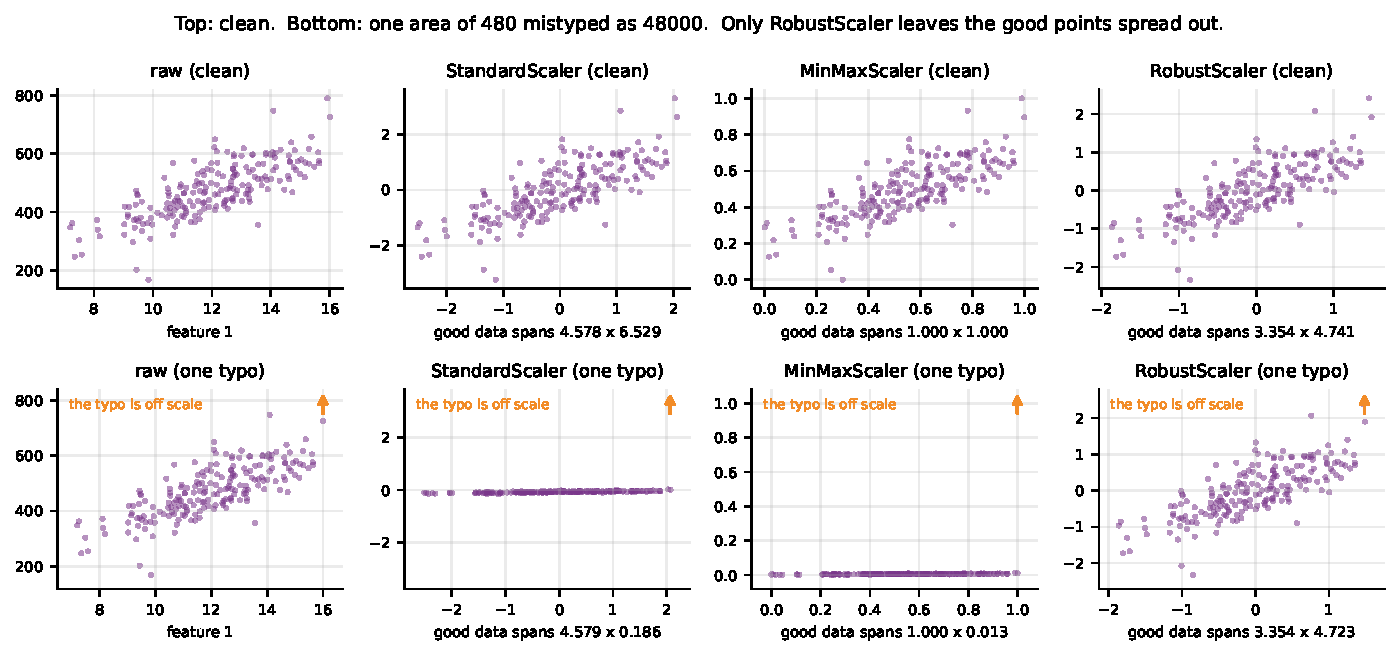
\includegraphics[width=0.86\textwidth]{scalers.pdf}
  \caption{Two hundred plots of land, with length on the horizontal axis and
  area on the vertical. Top row: clean. Bottom row: one area of $480$ typed as
  $48000$. The bottom frames are the \emph{same} frames as the top ones, so
  the collapse is visible; the typo itself is off scale. Under
  \texttt{MinMaxScaler} the good data ends up occupying $1.3\%$ of the unit
  interval.}
  \label{fig:scalers}
\end{figure}

\begin{caution}
\texttt{MinMaxScaler} is the dangerous one, because its output is
\emph{guaranteed} to be in $[0,1]$ and therefore looks correct. Nothing in the
output tells you that $99\%$ of your rows are inside a window of width
$0.013$. If you have not run an outlier check (Lecture~5), do not use
\texttt{MinMaxScaler}.
\end{caution}

\subsection{Which models change, measured}
\label{sec:whocares}

\begin{lstlisting}
cv = StratifiedKFold(5, shuffle=True, random_state=0)
for name, m in models:
    print(cross_val_score(m, Xb, yb, cv=cv).mean(),
          cross_val_score(make_pipeline(StandardScaler(), m), Xb, yb, cv=cv).mean())
\end{lstlisting}
\begin{codeout}
model                         raw   scaled   change
KNeighborsClassifier(5)    0.9315   0.9649  +0.0334
SVC(rbf)                   0.9210   0.9771  +0.0561
LogisticRegression         0.9543   0.9789  +0.0246
DecisionTreeClassifier     0.9262   0.9262  +0.0000
RandomForestClassifier     0.9649   0.9649  +0.0000
\end{codeout}

\begin{figure}[tb]
  \centering
  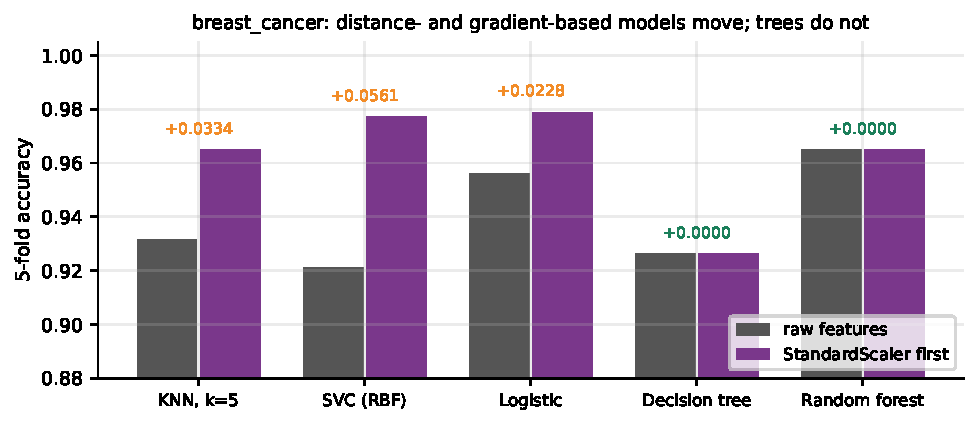
\includegraphics[width=0.66\textwidth]{scalescore.pdf}
  \caption{The same table drawn. The three left-hand pairs are models that
  measure a distance or descend a gradient; the two right-hand pairs are
  models that only ever ask which side of a threshold a value falls on.}
  \label{fig:scalescore}
\end{figure}

Those two zeros are not roundings. Here is the proof.

\begin{lstlisting}
t1 = DecisionTreeClassifier(random_state=0).fit(X_train, y_train)
sc = StandardScaler().fit(X_train)
t2 = DecisionTreeClassifier(random_state=0).fit(sc.transform(X_train), y_train)
np.array_equal(t1.tree_.feature, t2.tree_.feature)
\end{lstlisting}
\begin{codeout}
tree on raw    : 18 leaves, depth 5, test accuracy 0.902098
tree on scaled : 18 leaves, depth 5, test accuracy 0.902098
identical predictions on the test set: True
identical tree structure (same feature at every node): True
the thresholds differ, of course: raw 106.1000  scaled -0.0273 (same split)
\end{codeout}

\begin{keyidea}
A tree is invariant under any strictly increasing per-column transformation,
because every question it asks is about \emph{order}. Scaling a tree's inputs
is not wrong; it is simply a no-op that costs you the ability to read the
thresholds.
\end{keyidea}

\subsection{The gradient case}
\label{sec:gd}

\begin{lstlisting}
for eta in (1e-2, 1e-3, 1e-4, 1e-5, 1e-6):
    for X in (X_raw, StandardScaler().fit_transform(X_raw)):
        m = SGDRegressor(max_iter=50000, tol=1e-6, random_state=0,
                         learning_rate="constant", eta0=eta).fit(X, y)
        print(eta, m.n_iter_, m.score(X, y))
\end{lstlisting}
\begin{codeout}
eta0                          raw units                 standardised
0.01              6 epochs  R2 -1.7e+28        15 epochs  R2 +0.4951
0.001             6 epochs  R2 -4.8e+26        14 epochs  R2 +0.5142
0.0001            8 epochs  R2 -4.2e+25       184 epochs  R2 +0.5144
1e-05             24 epochs  R2 +0.2008       872 epochs  R2 +0.5139
1e-06             42 epochs  R2 +0.3478      5231 epochs  R2 +0.5113
ordinary least squares on the same data gives R2 +0.5177
condition number of X'X, raw          1.030e+06
condition number of X'X, standardised 4.701e+02
\end{codeout}

There is no step size at which the unscaled version works. Large steps diverge
--- an $R^2$ of $-1.7\times 10^{28}$ is an overflow, not a bad fit --- and small
steps stop early at $0.35$, because the tolerance is met while the shallow
direction has barely moved. Standardised, \emph{every} step size lands within
$0.007$ of least squares, the best in fourteen passes.

\begin{figure}[tb]
  \centering
  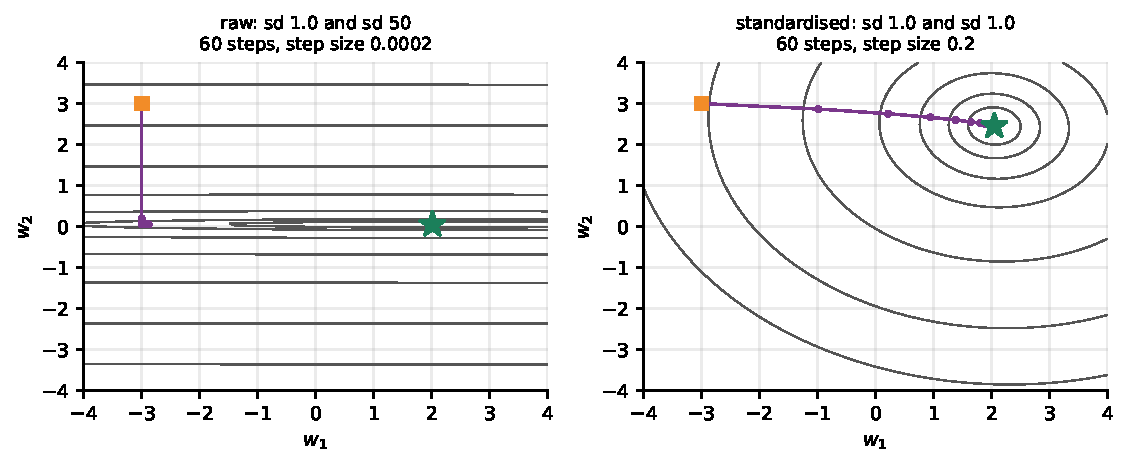
\includegraphics[width=0.70\textwidth]{gdpath.pdf}
  \caption{Two features, one with fifty times the spread of the other. Orange
  square is the start, green star the least-squares solution, purple the
  gradient-descent path. Left: Hessian condition number $2296.5$; after $60$
  steps the loss is $323$ times the optimum. Right: condition number $1.1$,
  and $60$ steps arrive.}
  \label{fig:gdpath}
\end{figure}

The condition number --- the ratio of the largest to the smallest eigenvalue of
$X^{\!\top}\!X$ --- is the quantitative version of that picture, and it bounds
how slowly gradient descent can converge. Standardising took it from a million
to four hundred and seventy.

\subsection{And the scaler is fitted on the training split}

Everything Lecture~5 said applies unchanged. \texttt{StandardScaler} learns two
numbers per column, \texttt{MinMaxScaler} learns two, \texttt{RobustScaler}
learns two. All of them must come from the training rows.

\begin{lstlisting}
# wrong
X_all = StandardScaler().fit_transform(X)
X_tr, X_te, y_tr, y_te = train_test_split(X_all, y, random_state=0)

# right
pipe = make_pipeline(StandardScaler(), KNeighborsClassifier())
cross_val_score(pipe, X, y, cv=5)
\end{lstlisting}

Lecture~5 measured the size of that leak: $+0.0034$ of accuracy with $20$
training rows, falling to $+0.0002$ with $427$. Real, and small. The much
larger leak of this lecture is in Section~\ref{sec:selectleak}.

\notesources{\AMLUnitIVSources}

% =========================================================================
\section{Feature encoding}
\label{sec:encode}

\subsection{Nominal and ordinal}

A categorical column is \textbf{ordinal} if its categories have a genuine
order --- \texttt{small} $<$ \texttt{medium} $<$ \texttt{large}, a degree
classification, a Likert response. It is \textbf{nominal} if they do not ---
colour, city, blood group, department, payment method.

There are two standard encodings. \textbf{Ordinal encoding} replaces each
category with an integer, giving one column. \textbf{One-hot encoding} creates
one $0/1$ column per category, with exactly one $1$ in each row.

\begin{keyidea}
Match the encoding to the variable, not to your convenience. Ordinal-encoding
a nominal variable asserts an order and a spacing that are not there, and a
linear model believes assertions.
\end{keyidea}

\subsection{Worked: what a linear model does with an ordinal code}
\label{sec:ordinalhand}

\begin{worked}[Three colours]
\texttt{OrdinalEncoder} sorts alphabetically, so \texttt{blue}$\,\to 0$,
\texttt{green}$\,\to 1$, \texttt{red}$\,\to 2$. Suppose the true mean target
for each colour is $20$, $50$ and $10$.

A linear model on the code column fits the best straight line through the
three points $(0, 20)$, $(1, 50)$, $(2, 10)$. With $\bar x = 1$ and
$\bar y = 80/3 = 26.667$:
\[
  S_{xy} = (-1)(-6.667) + (0)(23.333) + (1)(-16.667) = -10,
  \qquad S_{xx} = 1 + 0 + 1 = 2,
\]
so the slope is $-5$ and the intercept is $26.667 + 5 = 31.667$. The three
predictions are $31.667$, $26.667$, $21.667$ against truths of $20$, $50$,
$10$.
\[
  \mathrm{SSE} = 11.667^2 + 23.333^2 + 11.667^2 = 816.7, \qquad
  \mathrm{SST} = 6.667^2 + 23.333^2 + 16.667^2 = 866.7,
\]
\[
  R^2 = 1 - \frac{816.7}{866.7} = 0.0577 .
\]
The point is structural, not numerical. A straight line through codes
$0, 1, 2$ \emph{cannot} put the middle category highest, whatever its slope.
Ordinal coding has thrown away the ability to express the pattern.
\end{worked}

\begin{lstlisting}
rng = np.random.default_rng(0)          # the one seed for this lecture
colour = rng.choice(["blue", "green", "red"], size=900)
y = np.array([{"blue":20., "green":50., "red":10.}[c] for c in colour]) \
    + rng.normal(0, 2.0, 900)
ordc = OrdinalEncoder().fit_transform(colour.reshape(-1, 1))
ohc  = OneHotEncoder(sparse_output=False).fit_transform(colour.reshape(-1, 1))
\end{lstlisting}
\begin{codeout}
linear model, ordinal (1 column)   cross-validated R2 +0.0743
linear model, one-hot (3 columns)  cross-validated R2 +0.9868
a decision tree on the SAME ordinal column: accuracy 1.0000
\end{codeout}

$0.0743$ against $0.9868$, from a choice of encoder. The hand calculation
predicted $0.0577$; the difference is the noise we added. And once again
the third line matters: a tree on the ordinal column recovers the pattern
perfectly, because two splits on a code column separate three groups.
\textbf{The failure is a failure of the linear model plus that encoding, not
of the encoding alone.}

\begin{figure}[tb]
  \centering
  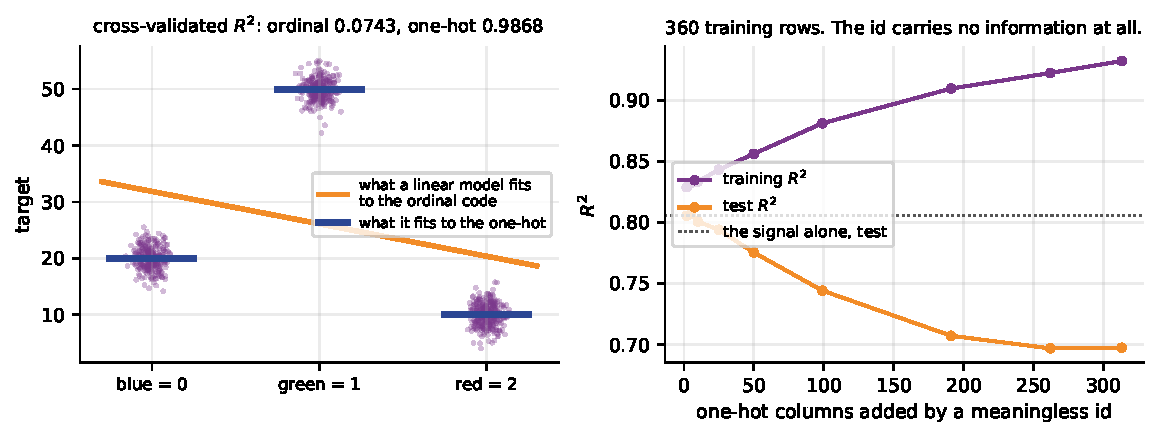
\includegraphics[width=0.86\textwidth]{encoding.pdf}
  \caption{Left: the orange line is the whole vocabulary a linear model has
  when given an ordinal code; the three blue bars are what one-hot lets it
  say. Right: the price of the opposite mistake, one-hot encoding an
  identifier that carries no information.}
  \label{fig:encoding}
\end{figure}

\subsection{The dummy variable trap}
\label{sec:trap}

If a design matrix has an intercept column of ones \emph{and} all $k$ dummy
columns, then the $k$ dummies sum to $1$ in every row, which is exactly the
intercept column. The matrix is rank-deficient and the coefficients are not
unique.

\begin{lstlisting}
D_full = np.c_[np.ones(900), OneHotEncoder(sparse_output=False).fit_transform(C)]
D_drop = np.c_[np.ones(900), OneHotEncoder(sparse_output=False,
                                           drop="first").fit_transform(C)]
print(np.linalg.matrix_rank(D_full), np.linalg.cond(D_full))
\end{lstlisting}
\begin{codeout}
with an intercept and all 3 dummies: shape (900, 4)  rank 3
   the three dummy columns sum to [1.] in every row
   condition number 3.436e+15
with an intercept and 2 dummies:     shape (900, 3)  rank 3
   condition number 3.810e+00
coefficients, all 3 dummies : [ 19.9581   0.0382  29.926  -10.0061]
a DIFFERENT coefficient vector: [ 119.9581  -99.9618  -70.074  -110.0061]
   same predictions? max difference 8.88e-15
both fit equally well: R2 0.986928 and 0.986928
\end{codeout}

The second coefficient vector was produced by adding $100$ to the intercept and
subtracting $100$ from each dummy. The predictions move by at most
$9 \times 10^{-15}$ --- floating-point dust on values near $20$ --- because the
change is $100 \times (1 - \sum_j \text{dummy}_j) = 0$ in every row.

\begin{caution}
Rank deficiency does not make your \emph{predictions} wrong --- both fits give
$R^2 = 0.986928$. It makes your \emph{coefficients} meaningless, and with them
every standard error, $t$-statistic and $p$-value. If anyone is going to
interpret the model, use \texttt{drop='first'}. Ridge, lasso and trees are
unaffected; ordinary least squares and statistical inference are not.
\end{caution}

Two practical notes: with ridge or lasso, dropping a level makes the penalty
asymmetric across the retained levels, so many practitioners keep all $k$; and
\texttt{drop='if\_binary'} is usually what you want for a mixed table.

\subsection{High cardinality}
\label{sec:cardinality}

One-hot encoding a column with $K$ levels adds $K$ columns. That is fine for
$K = 3$ and catastrophic for $K = 3000$.

\begin{codeout}
the id column has 256 distinct levels in 600 rows; one-hot makes 256 columns
signal only          train R2 +0.7586   test R2 +0.8063
signal + one-hot id  train R2 +0.8956   test R2 +0.6825
levels present in train but not test: 99
\end{codeout}

The identifier was generated at random and carries \emph{no} information about
the target. Adding it moved the training $R^2$ up by $0.14$ and the test $R^2$
down by $0.12$. Each dummy column fits a handful of rows exactly and predicts
nothing, which is a textbook picture of overfitting. And $82$ of the levels
never appear in the test set at all, so their coefficients were estimated from
data that will never recur.

What to do instead: group rare levels into a single \texttt{other}; use a
count or target encoding, fitted \emph{inside} the cross-validation fold like
any other learned quantity; or use a model with native categorical support.

\subsection{Two details that will bite you}
\label{sec:encdetails}

\begin{lstlisting}
enc = OneHotEncoder().fit([["small"], ["medium"], ["large"], ["small"]])
enc.transform([["extra-large"]])
\end{lstlisting}
\begin{codeout}
OneHotEncoder() default  ->  ValueError: Found unknown categories
   [np.str_('extra-large')] in column 0 during transform
handle_unknown='ignore'  ->  all-zero row:
[[0. 0. 1.]
 [0. 0. 0.]]
\end{codeout}

An unseen category at prediction time raises by default. \texttt{handle\_unknown
= 'ignore'} produces an all-zero row instead, which is a defensible choice
provided you know you have made it.

\begin{lstlisting}
OrdinalEncoder().fit_transform(sizes)                       # ALPHABETICAL
OrdinalEncoder(categories=[["small", "medium", "large"]])   # what you meant
\end{lstlisting}
\begin{codeout}
alphabetical (the default): [2. 1. 0. 1. 2.]
   categories_ = ['large' 'medium' 'small']
stated order              : [0. 1. 2. 1. 0.]
\end{codeout}

\begin{caution}
The default ordering put \texttt{large} before \texttt{medium}. If your
variable really is ordinal you must pass \texttt{categories=} explicitly; the
encoder cannot read English. This is a silent bug --- nothing raises, the model
fits, and the number it reports is simply worse than it should be.
\end{caution}

\notesources{\AMLUnitIVSources}

% =========================================================================
\section{Data reduction concepts}
\label{sec:reduce}

\subsection{Han, Kamber and Pei's three kinds}

\begin{center}
\begin{tabular}{@{}lp{4.4cm}p{5.2cm}@{}}
\toprule
& \textbf{What it removes} & \textbf{Methods}\\
\midrule
\textbf{Dimensionality reduction} & columns &
  attribute subset selection (Section~\ref{sec:select}), principal component
  analysis (Section~\ref{sec:pca}), wavelet transforms\\[4pt]
\textbf{Numerosity reduction} & rows, or the raw values &
  \emph{parametric}: fit a model and keep its parameters instead of the data;
  \emph{non-parametric}: histograms, clustering, sampling\\[4pt]
\textbf{Data compression} & bits &
  lossless (run-length and entropy coding); lossy (PCA and wavelets again,
  seen from the other side)\\
\bottomrule
\end{tabular}
\end{center}

The test that all three must pass is the same: \textbf{the reduced dataset must
support the same analysis and give substantially the same answer}, and the
reduction must cost less than the saving it produces.

\subsection{Why fewer columns: the curse of dimensionality}
\label{sec:curse}

\begin{lstlisting}
rng = np.random.default_rng(0)               # the one seed for this lecture
Q = rng.random((500, d))
D = np.sqrt(((Q[:, None, :] - Q[None, :, :]) ** 2).sum(-1))
np.fill_diagonal(D, np.inf);  near = D.min(axis=1)
np.fill_diagonal(D, -np.inf); far  = D.max(axis=1)
print(d, near.mean(), far.mean(), np.mean(far / near))
\end{lstlisting}
\begin{codeout}
    d mean dnear  mean dfar     dfar/dnear
    1     0.0010     0.7488      4425.9149
    2     0.0232     1.0332        67.5754
    5     0.2117     1.4525         7.3998
   10     0.5495     1.8870         3.5278
   50     2.1608     3.5227         1.6329
  100     3.3785     4.7283         1.4004
  500     8.4293     9.7936         1.1620
 1000    12.2254    13.6046         1.1129
\end{codeout}

At $d = 1000$ the farthest of the $499$ other points is only $1.11$ times as
far away as the nearest. Every pair of points is at very nearly the same
distance, so ``nearest neighbour'' has stopped carrying information.

\begin{figure}[tb]
  \centering
  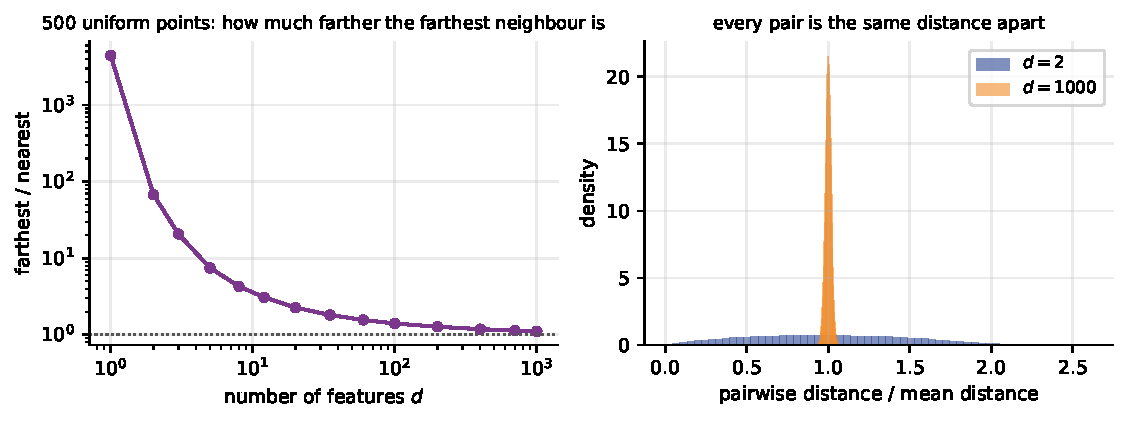
\includegraphics[width=0.76\textwidth]{curse.pdf}
  \caption{Left: the farthest-to-nearest ratio against $d$, log--log. Right:
  the whole distribution of pairwise distances at $d = 2$ and $d = 1000$, each
  divided by its own mean. At $d = 1000$ every distance in the dataset is
  within a few per cent of every other.}
  \label{fig:curse}
\end{figure}

\begin{keyidea}
Every method that measures a distance --- $k$-NN, $k$-means, RBF kernels,
DBSCAN --- degrades as the number of columns grows, and it degrades quietly.
Nothing in the output says ``the distances are meaningless now''.
\end{keyidea}

\subsection{Numerosity reduction: keep fewer rows}
\label{sec:sampling}

\begin{codeout}
digits, all 1797 rows               accuracy 0.9694
digits, a   50% sample ( 898 rows)  accuracy 0.9607  loss -0.0087
digits, a   25% sample ( 449 rows)  accuracy 0.9474  loss -0.0220
digits, a   10% sample ( 179 rows)  accuracy 0.9134  loss -0.0560
digits, a    5% sample (  89 rows)  accuracy 0.8506  loss -0.1188
\end{codeout}

Half the data costs under one point of accuracy; a twentieth costs twelve.
That shape --- flat at the top, steep at the bottom --- is the learning curve,
and it is the argument for the workflow you should adopt now: \textbf{prototype
on a sample, fit on everything}. It is also how you make a $200$-repetition
experiment finish before the lab period ends.

\notesources{\AMLUnitIVSources}

% =========================================================================
\section{Dimensionality reduction: principal component analysis}
\label{sec:pca}

\subsection{The question PCA asks}

Of all the directions in feature space, which one do the data vary along the
most? Then, among directions perpendicular to that one, which is next? And so
on. The recipe:

\begin{enumerate}[leftmargin=*]
  \item Centre every column by subtracting its mean, giving $X_c$.
  \item Form the covariance matrix
    $S = \frac{1}{n-1} X_c^{\!\top} X_c$.
  \item Compute the eigenvalues $\lambda_1 \ge \lambda_2 \ge \dots$ and their
    eigenvectors $u_1, u_2, \dots$ of $S$.
  \item Keep the top $k$. The \textbf{scores} are $T = X_c U_k$.
\end{enumerate}

Two facts make the whole thing readable. First, $\lambda_j$ \emph{is} the
variance of the data along component $j$, so
$\lambda_j / \sum_i \lambda_i$ is the \textbf{fraction of variance
explained}. Second, $\sum_i \lambda_i = \operatorname{tr}(S)$, the total
variance of the original columns --- a rotation moves variance around but
never creates or destroys it.

There is a second, equivalent characterisation that is often more useful:
\textbf{the $k$-dimensional subspace PCA finds is the one that minimises the
total squared reconstruction error.} Maximising retained variance and
minimising discarded variance are the same problem.

\subsection{Worked: five points in the plane}
\label{sec:pcahand}

\begin{worked}[PCA with no library at all]
Take $(1,2),\ (2,3),\ (3,5),\ (4,4),\ (5,6)$. The mean is $(3,4)$, so the
centred points are
\[
  (-2,-2),\quad (-1,-1),\quad (0,1),\quad (1,0),\quad (2,2).
\]
The sums of products are $\sum x_c^2 = 4+1+0+1+4 = 10$,
$\sum y_c^2 = 4+1+1+0+4 = 10$ and $\sum x_c y_c = 4+1+0+0+4 = 9$. Dividing by
$n - 1 = 4$:
\begin{equation}
  \label{eq:cov}
  S = \begin{pmatrix} 2.5 & 2.25 \\ 2.25 & 2.5 \end{pmatrix}.
\end{equation}
For a symmetric $2\times2$ matrix with \emph{equal} diagonal entries, the
eigenvectors are always $\frac{1}{\sqrt2}(1,1)$ and
$\frac{1}{\sqrt2}(1,-1)$: check by multiplying out,
$S\binom{1}{1} = \binom{4.75}{4.75}$. The eigenvalues are therefore
$2.5 + 2.25 = 4.75$ and $2.5 - 2.25 = 0.25$, so
\[
  \frac{\lambda_1}{\lambda_1 + \lambda_2} = \frac{4.75}{5.00} = 0.95,
  \qquad
  \frac{\lambda_2}{\lambda_1 + \lambda_2} = 0.05 .
\]
The trace checks: $2.5 + 2.5 = 5.0 = 4.75 + 0.25$.

The scores are the centred points dotted with $u_1$:
$-4/\sqrt2 = -2.8284$, $-1.4142$, $0.7071$, $0.7071$, $2.8284$. Their sample
variance is $(8 + 2 + 0.5 + 0.5 + 8)/4 = 4.75$, which is $\lambda_1$ ---
exactly as promised.
\end{worked}

\begin{figure}[tb]
  \centering
  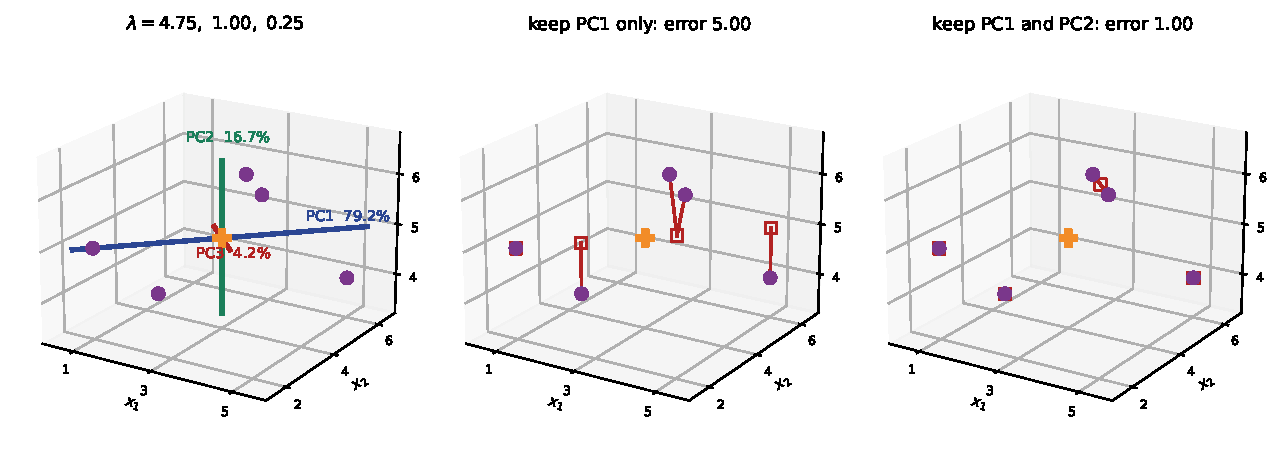
\includegraphics[width=0.64\textwidth]{pcahand.pdf}
  \caption{The five points, their mean, and the two eigenvectors drawn at
  length $\sqrt{\lambda_j}$. Right: each point projected onto PC1 alone. Only
  the two off-axis points move, by $\pm(0.5,-0.5)$, so the total squared
  reconstruction error is $1.0$.}
  \label{fig:pcahand}
\end{figure}

\begin{lstlisting}
S = np.cov(P - P.mean(axis=0), rowvar=False)
w, V = np.linalg.eigh(S)                     # by hand
p = PCA(n_components=2).fit(P)               # by library
p1 = PCA(n_components=1).fit(P)
R = p1.inverse_transform(p1.transform(P))
\end{lstlisting}
\begin{codeout}
covariance matrix
 [[2.5  2.25]
  [2.25 2.5 ]]
eigenvalues  [4.75 0.25]
sklearn explained_variance_ratio_ [0.95 0.05]
sklearn components_ (rows)
 [[ 0.707107  0.707107]
  [ 0.707107 -0.707107]]
reconstruction from 1 component [[1.0, 2.0], [2.0, 3.0], [3.5, 4.5], [3.5, 4.5], [5.0, 6.0]]
total squared reconstruction error 1.000000
check: (n-1) * lambda2 = 4 * 0.2500 = 1.000000
\end{codeout}

Two things to notice. The points $(3,5)$ and $(4,4)$ both reconstruct to
$(3.5, 4.5)$: dropping a component \textbf{merges points that differed only
along it}, which is what ``lossy'' means. And the reconstruction error is
exactly $(n-1)\lambda_2$, which is the general identity of the next section.

\subsection{The reconstruction identity, and choosing $k$}
\label{sec:recon}

Write the centred data in the eigenbasis: $x_c = \sum_j t_j u_j$ with
$t_j = x_c^{\!\top} u_j$. Keeping the top $k$ components means setting
$t_{k+1}, \dots, t_d$ to zero, so the squared error for that point is
$\sum_{j>k} t_j^2$. Summing over all $n$ points and using
$\sum_i t_{ij}^2 = (n-1)\lambda_j$:
\begin{equation}
  \label{eq:recon}
  \text{total squared reconstruction error} = (n-1)\sum_{j > k} \lambda_j ,
  \qquad
  \frac{\text{error}}{\text{total}} = 1 - \frac{\sum_{j\le k}\lambda_j}
                                              {\sum_{j}\lambda_j}.
\end{equation}
So \emph{variance kept} and \emph{relative error removed} add to exactly one.
That is why a single curve answers both questions.

\begin{codeout}
breast_cancer, standardised, 30 features
    1 components explain  44.27%      80% needs  5 components (16.7% of 30)
    2 components explain  63.24%      90% needs  7 components (23.3% of 30)
    5 components explain  84.73%      95% needs 10 components (33.3% of 30)
   10 components explain  95.16%      99% needs 17 components (56.7% of 30)
digits, standardised, 64 features
   80% needs 21   90% needs 31   95% needs 40   99% needs 54  of 64
\end{codeout}

\begin{figure}[tb]
  \centering
  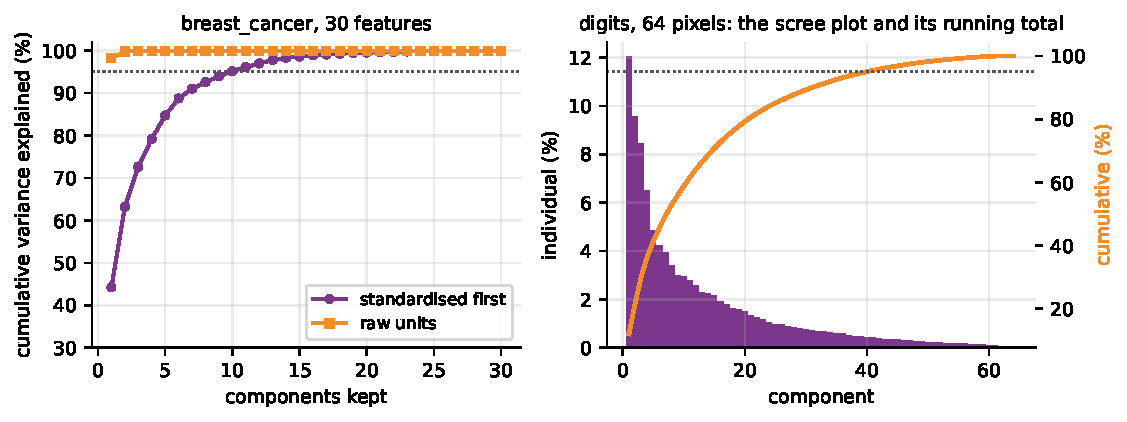
\includegraphics[width=0.80\textwidth]{pcavar.pdf}
  \caption{Left: cumulative variance explained for breast\_cancer, with and
  without standardising first. Right: the digits scree plot with its running
  total on the right-hand axis.}
  \label{fig:pcavar}
\end{figure}

\begin{caution}
There is no universal ``keep $95\%$'' rule. On breast\_cancer that is ten of
thirty columns, because the thirty features are ten measurements each recorded
three ways and are therefore heavily redundant. On digits it is forty of
sixty-four. \textbf{$95\%$ of what depends entirely on the data.} An elbow in
the scree plot is a suggestion, not a criterion; if $k$ matters to your score,
choose it by cross-validation like any other hyper-parameter.
\end{caution}

The reconstruction is worth seeing rather than reading.

\begin{codeout}
digits, PCA reconstruction error against k
   k= 1  variance kept  14.89%  relative reconstruction error  85.11%
   k= 2  variance kept  28.51%  relative reconstruction error  71.49%
   k= 5  variance kept  54.50%  relative reconstruction error  45.50%
   k=10  variance kept  73.82%  relative reconstruction error  26.18%
   k=20  variance kept  89.43%  relative reconstruction error  10.57%
   k=30  variance kept  95.91%  relative reconstruction error   4.09%
   k=40  variance kept  98.82%  relative reconstruction error   1.18%
   k=64  variance kept 100.00%  relative reconstruction error   0.00%
\end{codeout}

Every row sums to $100\%$, which is Equation~\eqref{eq:recon} checked
numerically eight times.

\begin{figure}[tb]
  \centering
  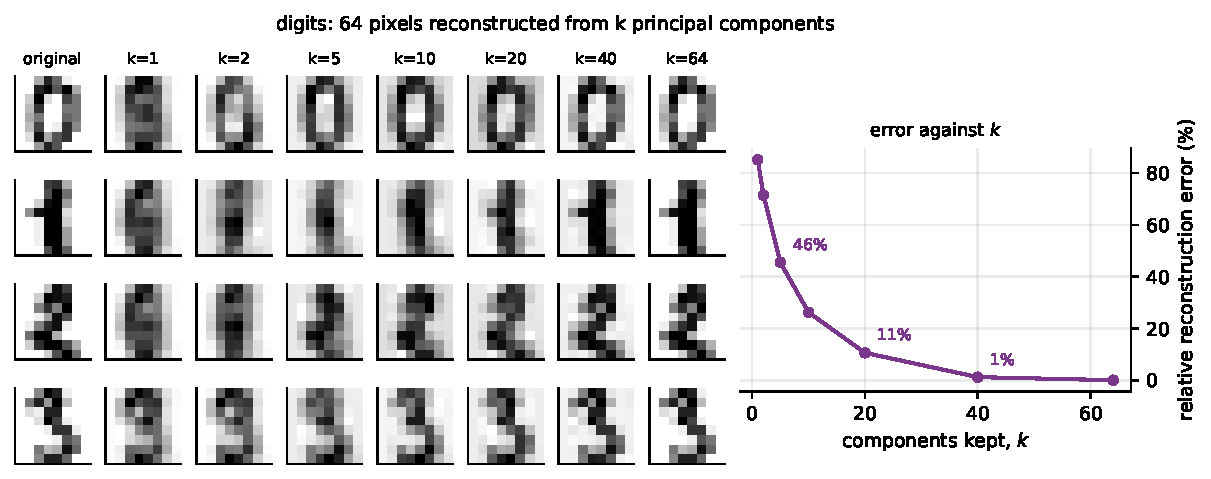
\includegraphics[width=0.90\textwidth]{pcarecon.pdf}
  \caption{Four digits reconstructed from $k$ principal components. At
  $k = 5$ you can tell a $0$ from a $1$; at $k = 20$ they are all legible and
  $44$ of the $64$ numbers per image have been discarded.}
  \label{fig:pcarecon}
\end{figure}

\subsection{Scale before you rotate}
\label{sec:pcascale}

\begin{codeout}
PCA on breast_cancer WITHOUT scaling
   PC1 explains 0.9820 of the variance
   its largest loading is 0.8521 on 'worst area'
   that feature's standard deviation is 568.9; the smallest in the table is 0.00264
PCA on breast_cancer WITH StandardScaler
   PC1 explains 0.4427 of the variance
   its largest loading is 0.2609 on 'mean concave points'
\end{codeout}

Unscaled, the first component explains $98.20\%$ of the variance and is
essentially the \texttt{worst area} column with a new name. That is not a
discovery; it is the definition of PCA meeting a table whose columns have
different units. Variance has units, and the widest column wins by
construction.

\begin{keyidea}
Standardise before PCA unless every column is already measured in the same
unit. Otherwise you have run an eigendecomposition to find out which of your
columns you recorded in the biggest numbers.
\end{keyidea}

\subsection{PCA is not feature selection}
\label{sec:pcanotselect}

\begin{codeout}
PC1 of the standardised breast_cancer data: 30 loadings
   largest  |loading| 0.2609    smallest |loading| 0.0145
   number of features with |loading| > 0.10 : 26 of 30
   number needed to reach 90% of the loading vector's length: 20
      +0.2609  mean concave points    +0.2584  mean concavity
      +0.2509  worst concave points   +0.2393  mean compactness
to compute PC1 for a new patient you need ALL 30 measurements.
\end{codeout}

\begin{figure}[tb]
  \centering
  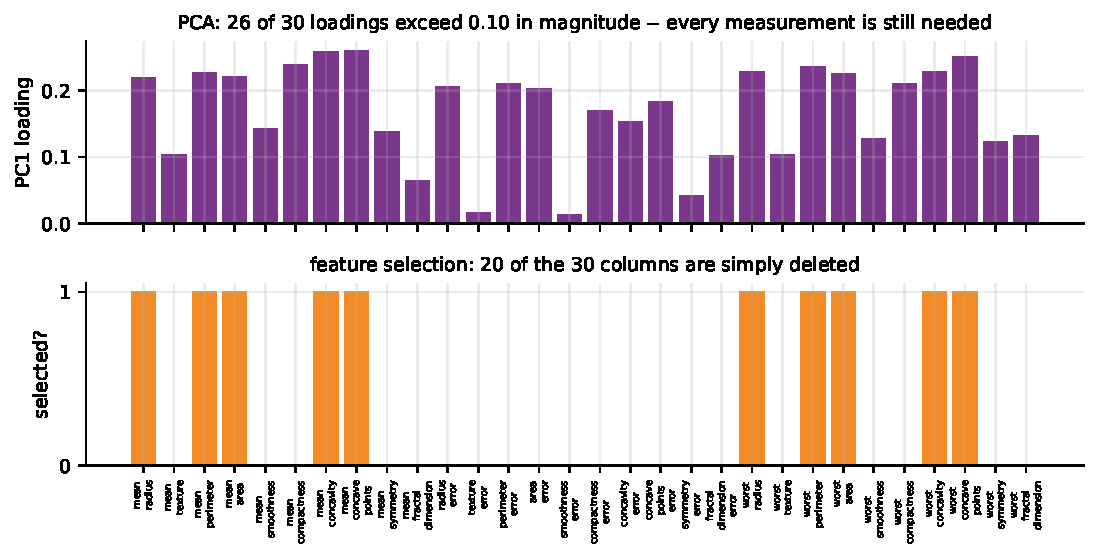
\includegraphics[width=0.76\textwidth]{pcaload.pdf}
  \caption{Top: the thirty PC1 loadings, twenty-six of them above $0.10$ in
  magnitude. Bottom: what a filter selecting ten features does to the same
  thirty columns. One rotates; the other deletes.}
  \label{fig:pcaload}
\end{figure}

\begin{caution}
``I reduced to ten components'' does not mean ``I only need ten
measurements''. Every component is a weighted sum of all thirty original
columns, so the cost of collecting one row is unchanged. \textbf{If your reason
for reducing was that a test is expensive or invasive, PCA has not helped you
at all}; feature selection has. And
$0.2609 \times \texttt{concave points} + 0.2584 \times \texttt{concavity} +
\cdots$ is not a quantity a clinician can name, so interpretability is gone
too.
\end{caution}

\subsection{PCA has never heard of your labels}
\label{sec:pcaunsup}

\begin{lstlisting}
rng   = np.random.default_rng(0)     # the one seed for this lecture
big   = rng.normal(0, 10.0, 600)     # huge variance, no signal
small = rng.normal(0,  1.0, 600)     # small variance, IS the label
y = (small > 0).astype(int)
X = np.c_[big, small]
\end{lstlisting}
\begin{codeout}
PC1 explains 0.9909 of the variance; its loadings are [1.     0.0052]
logistic regression on both features        accuracy 0.9850
logistic regression on PCA's 1 component    accuracy 0.5200
logistic regression on the 1 feature a filter would pick  0.9933
after standardising first, PCA's component  accuracy 0.7617
\end{codeout}

PCA discarded the only informative direction and kept the noise, taking the
accuracy from $0.9850$ to a coin flip. Standardising first helps a little
($0.7617$) but does not fix it, because the problem is not the units --- it is
that $y$ was never consulted. A supervised filter picking one column scored
$0.9933$.

\begin{keyidea}
PCA is \textbf{unsupervised}: it maximises variance, and variance is not
relevance. In practice it usually works, because on real data the directions
that vary most usually do carry the signal --- but ``usually'' is not
``always'', and you should check rather than assume.
\end{keyidea}

Two named alternatives worth knowing. \textbf{Linear discriminant analysis}
finds directions that separate the \emph{classes} rather than maximising
variance, and would solve the example above. \textbf{Partial least squares}
(ISLP \S6.3) does the analogous thing for regression. Both are supervised, and
both therefore must be fitted inside the fold.

\subsection{PCA is fitted on the training split}
\label{sec:pcaleak}

\begin{codeout}
  components whose sign flipped between the two fits: 3.0 of 10, up to 6
  correct                  accuracy 0.9768  +/- 0.0128   worst split 0.9357
  fit on everything        accuracy 0.9773  +/- 0.0122   worst split 0.9415
  refit on the test set    accuracy 0.9447  +/- 0.0226   worst split 0.8947
  refitting on the test set costs -0.0320 on average and -0.0877 on the
  worst of the 40 splits
  fit-on-everything minus correct: +0.0006  t +0.94  wins 8/40
\end{codeout}

Be honest about which of the two mistakes is which. Fitting the scaler and PCA
on all the rows before splitting leaked \textbf{nothing measurable} here:
$+0.0006$ with $t = 0.94$ over $40$ splits, and the leaky version won on only
$8$ of them. That is what we should expect --- PCA never sees $y$, so the only
thing it can absorb from the test rows is a little information about the
covariance structure.

Calling \texttt{fit\_transform} \emph{again} on the test set is a different and
much worse error, and it is the one students actually make. The test
components are a different basis: on average three of the ten point the
opposite way, so ``column 3'' in training and ``column 3'' at test time are
not the same feature. That cost $-0.0320$ on average, and $-0.0877$ on the
worst of the forty splits.

\begin{caution}
Use \texttt{fit\_transform} on the training data and \texttt{transform}
--- never \texttt{fit\_transform} --- on anything else. A \texttt{Pipeline}
enforces this for you, which is the entire reason it exists.
\end{caution}

The reason PCA leaks so little is the one Section~\ref{sec:pcaunsup} gave: it
is unsupervised. The step that leaks a great deal is the one that \emph{does}
look at $y$, and it is next.

\notesources{\AMLUnitIVSources}

% =========================================================================
\section{Feature selection}
\label{sec:select}

\subsection{Three families}

\begin{center}
\begin{tabular}{@{}lp{4.6cm}p{4.8cm}@{}}
\toprule
& \textbf{How it decides} & \textbf{Cost and risk}\\
\midrule
\textbf{Filter} & a statistic per feature, computed once, model ignored:
  variance, ANOVA $F$, mutual information, correlation, $\chi^2$ &
  cheapest; blind to interactions and to redundancy between features\\[5pt]
\textbf{Wrapper} & fit the model repeatedly and keep what helps: forward
  selection, backward elimination, recursive feature elimination &
  most expensive; can overfit the selection itself\\[5pt]
\textbf{Embedded} & the model selects while it fits: L1 (lasso), tree
  importances & nearly free; the answer is specific to that model\\
\bottomrule
\end{tabular}
\end{center}

Han, Kamber and Pei call this \textbf{attribute subset selection}, and list it
under dimensionality reduction alongside PCA. The difference from PCA is the
one Section~\ref{sec:pcanotselect} made: selection deletes columns, so the row
you have to collect gets cheaper and the model stays readable.

\subsection{Filter, part 1: variance}
\label{sec:variance}

\begin{lstlisting}
VarianceThreshold(threshold=0.0).fit(Xg)
\end{lstlisting}
\begin{codeout}
digits: 3 of the 64 pixels have zero variance (always the same value)
        48 of the 64 survive a variance threshold of 1.0
logistic regression on all 64 pixels          accuracy 0.9694
      threshold   0.0 keeps 61 pixels            accuracy 0.9694
      threshold   1.0 keeps 48 pixels            accuracy 0.9694
      threshold  10.0 keeps 43 pixels            accuracy 0.9683
\end{codeout}

Sixteen of the sixty-four columns removed for nothing at all, and twenty-one
for $0.0011$. A variance filter almost never improves a score --- what it buys
is \textbf{columns}. It
is also a correctness measure rather than a performance one: a constant column
makes \texttt{StandardScaler} divide by zero and makes every correlation with
it undefined.

Note the unit problem: variance has units, so a threshold of $1.0$ means
something different for metres and for millimetres. Threshold each column
relative to its own scale, or use a scale-free filter.

\subsection{Filter, part 2: the $F$ test and mutual information disagree}
\label{sec:filters}

The ANOVA $F$ statistic for classification compares the \emph{class means} of
a feature. Mutual information estimates $I(X_j; Y)$ and makes no assumption
about the form of the dependence. Where the dependence is not a difference of
means, they part company.

\begin{lstlisting}
rng = np.random.default_rng(0)            # the one seed for this lecture
a = rng.normal(0, 1, 1000)                # enters the label linearly
b = rng.normal(0, 1, 1000)                # enters only through |b|
noise = rng.normal(0, 1, (1000, 8))
lab = ((a + (np.abs(b) - 0.8) * 2.0 + rng.normal(0, 0.4, 1000)) > 0).astype(int)
\end{lstlisting}
\begin{codeout}
feature             ANOVA F     rank  mutual info     rank
a (linear)          317.110        1       0.1342        2
b (|b| only)          0.213        8       0.2263        1
best noise            8.326        -       0.0123        -
b ranks 8 of 10 by F and 1 of 10 by mutual information.
SelectKBest(f_classif, k=3)           picks ['a', 'noise 1', 'noise 2']
SelectKBest(mutual_info_classif, k=3) picks ['a', 'b', 'noise 8']
\end{codeout}

The two classes have the same mean $b$ --- the label depends on $|b|$, which is
symmetric --- so the $F$ test sees an $F$ of $0.213$ and ranks the genuinely
informative feature \emph{eighth of ten}, below six of the eight noise
columns. Mutual information ranks it first.

\begin{keyidea}
A filter measures the kind of dependence it was built to measure, and nothing
else. Choosing a filter is choosing an assumption about how features relate to
the target.
\end{keyidea}

There is a price, and it is worth stating in a form that does not depend on
the machine. Mutual information is non-parametric: for every one of the $30$
columns, in every one of the $5$ folds, it runs a nearest-neighbour search
--- $150$ searches --- where the $F$ test needs two sums per column. It also
needs more rows to estimate reliably. On the machine these notes were built
on that came to $0.23$ seconds against $0.02$; on yours it will be different
numbers with the same ordering.

\subsection{Wrapper: recursive feature elimination}
\label{sec:rfe}

Fit the model. Drop the feature with the smallest coefficient. Refit on what
remains. Repeat. With \texttt{step=1} on $30$ features that is $30$ model fits.

\begin{lstlisting}
RFE(LogisticRegression(max_iter=5000), n_features_to_select=10).fit(Z, y)
\end{lstlisting}
\begin{codeout}
30 features with step=1 means 30 fits.
elimination order, first six      the last one standing: worst area
   dropped 30 of 30: worst compactness      dropped 27: mean smoothness
   dropped 29 of 30: mean symmetry          dropped 26: texture error
   dropped 28 of 30: concavity error        dropped 25: concave points error
   RFE k= 1  accuracy 0.9157      RFE k=10  accuracy 0.9684
   RFE k= 2  accuracy 0.9526      RFE k=20  accuracy 0.9789
   RFE k= 5  accuracy 0.9684      RFE k=30  accuracy 0.9789
   RFECV picks its own k: 26 features, accuracy 0.9824
\end{codeout}

A wrapper asks the \emph{model} what it needs, so it can see redundancy that a
univariate filter cannot: if two columns carry the same information, a filter
scores both highly and keeps both, while RFE drops one as soon as the other is
present. The price is a model fit per step, and the answer is that model's
answer --- RFE with a logistic regression and RFE with a random forest will
disagree.

\texttt{RFECV} runs RFE inside a cross-validation loop and picks the $k$ that
maximises the score. Left to itself it kept \textbf{$26$ of the $30$}, which
is the first hint of Section~\ref{sec:doesithelp}.

\subsection{Embedded: L1 shrinks coefficients to exactly zero}
\label{sec:l1}

\begin{lstlisting}
for alpha in (0.01, 0.1, 0.5, 1.0, 2.0, 5.0, 20.0):
    la = Lasso(alpha=alpha).fit(StandardScaler().fit_transform(Xd), yd)
    print(alpha, (la.coef_ != 0).sum())
\end{lstlisting}
\begin{codeout}
   alpha  0.01  10 nonzero  CV R2 +0.4823
   alpha  0.10   9 nonzero  CV R2 +0.4825
   alpha  0.50   8 nonzero  CV R2 +0.4818
   alpha  1.00   7 nonzero  CV R2 +0.4820
   alpha  2.00   7 nonzero  CV R2 +0.4798
   alpha  5.00   5 nonzero  CV R2 +0.4659  sex,bmi,bp,s3,s5
   alpha 20.00   3 nonzero  CV R2 +0.3492  bmi,bp,s5
   ridge alpha 1.00  10 nonzero  CV R2 +0.4822
\end{codeout}

Five features of ten retain $97\%$ of the $R^2$; three retain $72\%$. The
lasso hands you the whole trade-off curve for free and $\alpha$ is the dial.
Ridge with the same $\alpha$ keeps all ten and scores the same: \textbf{L1
selects, L2 shrinks.} Because the selection depends on $\alpha$, the selection
is a hyper-parameter and belongs inside the cross-validation loop like any
other.

\subsection{The four selectors do not agree}
\label{sec:disagree}

\begin{codeout}
ANOVA F       picked 10: [0, 2, 3, 6, 7, 20, 22, 23, 26, 27]
mutual info   picked 10: [0, 2, 3, 6, 7, 13, 20, 22, 23, 27]
RFE           picked 10: [7, 10, 13, 15, 20, 21, 22, 23, 26, 27]
L1 logistic   picked  8: [7, 10, 20, 21, 24, 26, 27, 28]

pairwise overlap (Jaccard)
   ANOVA F       vs mutual info    9 shared, Jaccard 0.82
   ANOVA F       vs RFE            6 shared, Jaccard 0.43
   ANOVA F       vs L1 logistic    4 shared, Jaccard 0.29
   mutual info   vs RFE            6 shared, Jaccard 0.43
   mutual info   vs L1 logistic    3 shared, Jaccard 0.20
   RFE           vs L1 logistic    6 shared, Jaccard 0.50

chosen by all four: mean concave points, worst radius, worst concave points
chosen by at least one: 16 of 30 features
\end{codeout}

Three features of thirty command a consensus. The two filters agree with each
other ($0.82$) and with nobody else, which makes sense --- they are both
univariate. Sixteen of the thirty columns were picked by somebody.

\begin{keyidea}
There is no such thing as ``the important features''. There is only ``the
features that this criterion, with this model, at this $k$, chose''. Report
the criterion whenever you report a selection.
\end{keyidea}

\begin{figure}[tb]
  \centering
  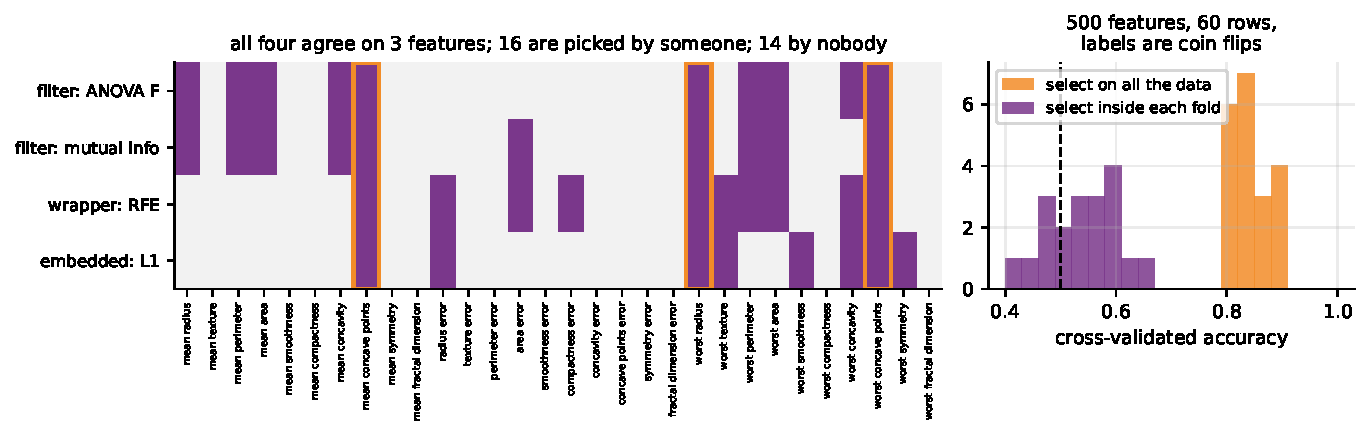
\includegraphics[width=0.92\textwidth]{selection.pdf}
  \caption{Left: the four selectors against the thirty breast\_cancer
  features; orange boxes mark the three on which all four agree. Right: the
  same experiment on the same random data, differing only in whether the
  selector was fitted inside the fold.}
  \label{fig:selection}
\end{figure}

\subsection{Does selection help? Report the experiment honestly}
\label{sec:doesithelp}

\begin{codeout}
selector                   accuracy
all 30 features              0.9789
filter: ANOVA F, k=10        0.9596
filter: mutual info, k=10    0.9561
wrapper: RFE, k=10           0.9684
embedded: L1, C=0.08         0.9719
cost in counts, which are the same on every machine:
   RFE k=10      21 model fits per fold (30 features down to 10, one at a
                 time) = 105 fits over 5 folds
   ANOVA F k=10   1 model fit per fold =   5 fits over 5 folds, so RFE costs
                 21 times as many fits
\end{codeout}

Not one of the four beat simply using all thirty columns. RFE, at $21$ model
fits per fold against the filter's one, recovered the most of the loss. This
is not a failure of the experiment; it is the answer.

\begin{caution}[Count fits, not seconds]
Everything else in these notes reproduces exactly. The seconds do not: they
depend on your processor, your BLAS build and what else is running, and the
same comparison on the same machine varies from run to run. So the cost claim
above is stated in \emph{model fits} --- $21$ per fold against $1$, true on
every machine --- and the seconds are reported only as a labelled measurement.
If you time it and get a different ratio, you are not wrong.
\end{caution}

\begin{caution}
Do not select features because you were told that selecting features is good
practice. Select when you need a cheaper row to collect, a model somebody has
to read, a model small enough to deploy, or when $d$ is large relative to $n$.
At $569 \times 30$, breast\_cancer is none of those things.
\end{caution}

\subsection{Selecting with the labels, before the split}
\label{sec:selectleak}

This is the centrepiece of the lecture.

\begin{lstlisting}
for rep in range(20):                    # a sweep: 20 different draws
    rng = np.random.default_rng(100 + rep)
    Xr = rng.normal(size=(60, 500))      # pure noise
    yr = rng.integers(0, 2, 60)          # labels are coin flips

    # wrong: score every feature on ALL the data, then cross-validate
    f, _ = f_classif(Xr, yr)
    keep = np.argsort(-f)[:20]
    cross_val_score(LogisticRegression(), Xr[:, keep], yr, cv=5).mean()

    # right: the selector is a step in the Pipeline
    cross_val_score(Pipeline([("sel", SelectKBest(f_classif, k=20)),
                              ("lr",  LogisticRegression())]),
                    Xr, yr, cv=5).mean()
\end{lstlisting}
\begin{codeout}
500 features, 60 rows, labels are pure coin flips. Truth is 0.5000.
   select on ALL the data, then cross-validate : 0.8475  +/- 0.0293
   select INSIDE each fold (Pipeline)          : 0.5342  +/- 0.0710
   overstatement                                +0.3133
   the wrong way beat 0.5 on 20 of 20 repetitions
\end{codeout}

There is nothing to learn in this dataset. The honest answer is $0.5$. The
first procedure reports $0.85$, every single time.

The mechanism is worth stating slowly. With $500$ candidates and $60$ rows,
some features correlate with the labels by chance --- that is what $500$ tries
at a coin-flipping game buys you --- and the $F$ test finds them. But it found
them \emph{using the labels of every row, including the rows that will shortly
be held out}. By the time cross-validation runs, the held-out rows have already
voted on which columns are in the model.

\begin{keyidea}
Any step that looks at $y$ is part of the model and must be refitted inside
every fold. Scaling and PCA leak little because they never see $y$. Feature
selection sees $y$, and it leaked $+0.3133$.
\end{keyidea}

This is the classic error described in Hastie, Tibshirani and Friedman's
\emph{Elements of Statistical Learning} \S7.10.2 as ``the wrong way to do
cross-validation''; it is the reason a great many published results in
high-dimensional biology did not replicate.

\subsection{Everything in one pipeline}
\label{sec:pipeline}

\begin{lstlisting}
pipe = Pipeline([
    ("scale",  StandardScaler()),
    ("select", SelectKBest(f_classif, k=15)),
    ("pca",    PCA(n_components=8)),
    ("model",  LogisticRegression(max_iter=5000)),
])
cross_val_score(pipe, Xb, yb, cv=5).mean()
\end{lstlisting}
\begin{codeout}
scale -> select 15 -> PCA to 8 -> logistic regression
   5-fold accuracy 0.9490  +/- 0.0140
   compare: raw logistic regression, all 30 features 0.9789
\end{codeout}

The mean and standard deviation of each column, the fifteen chosen columns and
the eight rotation directions are all recomputed inside every fold from four
fifths of the data. Nothing leaks.

And read the second line, because it is the honest end of the lecture: the
four-step pipeline scored \emph{worse} than doing nothing at all. It cannot
leak, and it also did not help. Both facts are worth reporting.

\notesources{\AMLUnitIVSources}

% =========================================================================
\section{Summary}

\begin{enumerate}[leftmargin=*]
  \item A representation is good only relative to a model. One engineered
    product column took a linear model from $R^2 = 0.9091$ to $0.9981$; a
    random forest reached the same place unaided. Binning bought a linear
    model $+0.0957$ and cost a tree $-0.0323$, and afterwards both fitted
    exactly the same step function.
  \item \texttt{PolynomialFeatures} degree $3$ turns $30$ columns into $5455$.
    On diabetes, degree $2$ cost $-0.0643$ of $R^2$ even with ridge.
  \item Age against income: the income column supplied $99.995\%$ of the
    squared distance, and standardising \textbf{changed which customer was the
    nearest neighbour}.
  \item Scaling was worth $+0.0561$ to an RBF SVM, $+0.0334$ to $k$-NN,
    $+0.0246$ to logistic regression, and \textbf{exactly $0.0000$} to a
    decision tree and a random forest --- the same tree, node for node,
    because a split is a question about order.
  \item Unscaled, stochastic gradient descent diverged at every usable step
    size ($R^2 = -1.7\times10^{28}$) and stalled at $0.35$ at the small ones.
    Standardised, it reached $0.5144$ against a least-squares $0.5177$ in
    fourteen epochs. Condition number: $1.03\times10^{6}$ against $470$.
  \item One typo squeezed the good data $78\times$ under
    \texttt{StandardScaler}, $71\times$ under \texttt{MinMaxScaler} and
    $2\times$ under \texttt{RobustScaler}.
  \item Ordinal-coding a nominal variable gave $R^2 = 0.0743$ against $0.9868$
    for one-hot; the hand calculation predicted $0.0577$, and a tree on the
    same ordinal column got $1.0000$. An intercept plus all $k$ dummies is
    rank-deficient (condition number $3.4\times10^{15}$), and two completely
    different coefficient vectors gave identical predictions.
  \item One-hot encoding a $256$-level identifier that carried no information
    moved the training $R^2$ up $0.14$ and the test $R^2$ down $0.12$.
  \item In $1000$ dimensions the farthest of $499$ points is only $1.11\times$
    as far as the nearest. Sampling half the digits rows cost $0.0087$ of
    accuracy; sampling a twentieth cost $0.1188$.
  \item PCA on unscaled breast\_cancer: PC1 explained $98.20\%$ and was the
    widest column. Standardised: $44.27\%$, and $95\%$ needed $10$ of $30$
    components --- but $40$ of $64$ on digits. Variance kept and relative
    reconstruction error always sum to $100\%$.
  \item PCA is a rotation, not a selection: $26$ of $30$ loadings exceed
    $0.10$, so all thirty measurements are still needed. And it is
    unsupervised --- it took an accuracy of $0.9850$ down to $0.5200$ by
    discarding the only informative direction.
  \item Refitting PCA on the test set cost $-0.0320$ on average and
    $-0.0877$ at worst; fitting it on all the
    rows before splitting cost nothing measurable ($t = 0.94$).
    \textbf{Selecting features with the labels before cross-validating scored
    $0.8475$ on pure coin flips, against $0.5342$ inside a
    \texttt{Pipeline}.}
  \item None of the four selectors beat using all thirty features on
    breast\_cancer, and \texttt{RFECV} chose to keep $26$ of them. Report that
    kind of result rather than hiding it.
\end{enumerate}

% =========================================================================
\section{Practice questions}

Attempt these before reading Section~\ref{sec:solutions}. Questions 1, 2, 3, 5
and 6 are pure hand arithmetic and are the ones most likely to appear on a
paper.

\begin{enumerate}[leftmargin=*]
  \item\label{q:scale} A column contains $10,\ 20,\ 30,\ 40,\ 100$. (a)
    Compute its mean, population standard deviation, minimum, maximum, median,
    $Q_1$, $Q_3$ and IQR. (b) Write out the column after
    \texttt{StandardScaler}, \texttt{MinMaxScaler} and \texttt{RobustScaler}.
    (c) What fraction of the $[0,1]$ interval do the first four values occupy
    after min--max scaling, and what does that imply for a $k$-NN model?

  \item\label{q:dist} Three people are recorded as height in cm, weight in kg
    and hours of exercise per week:
    $P = (170, 60, 3)$, $Q = (155, 62, 9)$, $R = (172, 85, 4)$. (a) Compute
    $d(P,Q)^2$ and $d(P,R)^2$ on the raw numbers, showing the contribution of
    each column. (b) Standardise each column and repeat. (c) Which point is
    $P$'s nearest neighbour in each case, and which answer would you defend?

  \item\label{q:encode} A nominal column \texttt{region} takes the values
    \texttt{north}, \texttt{south}, \texttt{east}, \texttt{west}, whose mean
    targets are $40$, $40$, $10$, $10$ respectively. (a) Write down the codes
    \texttt{OrdinalEncoder} will assign with its default settings. (b) Fit the
    best straight line through the four (code, mean) points by hand and give
    its $R^2$. (c) What is the $R^2$ of a one-hot fit? (d) If you one-hot
    encode all four levels and include an intercept, what is the rank of the
    resulting $4 \times 5$ design matrix, and why does that matter?

  \item\label{q:ordinal} You have a column of shirt sizes
    \texttt{small}, \texttt{medium}, \texttt{large} and you write
    \texttt{OrdinalEncoder().fit\_transform(sizes)}. What codes do you get, and
    why? Give the one-line fix. Why does nothing raise an error?

  \item\label{q:card} A table has three nominal columns with $50$ levels each
    and $2000$ rows. (a) How many columns after one-hot encoding, with and
    without \texttt{drop='first'}? (b) How many degree-2 interaction terms
    would \texttt{PolynomialFeatures} then generate from those one-hot columns
    alone? (c) Given the measured result of Section~\ref{sec:cardinality},
    what would you do instead?

  \item\label{q:pca} A centred two-feature dataset has covariance matrix
    $S = \begin{pmatrix} 4 & 2\\ 2 & 4\end{pmatrix}$. (a) Find both
    eigenvalues and eigenvectors by hand. (b) What fraction of the variance
    does PC1 explain? (c) Check your eigenvalues against the trace. (d) If the
    dataset has $n = 21$ points, what is the total squared reconstruction
    error from keeping only PC1?

  \item\label{q:recon} Prove Equation~\eqref{eq:recon}: that the total squared
    reconstruction error from keeping the top $k$ components is
    $(n-1)\sum_{j>k}\lambda_j$. Then use the digits table in
    Section~\ref{sec:recon} to state, without any further computation, the
    variance explained by the top $20$ of the $64$ components.

  \item\label{q:vspca} You must reduce a $40$-column clinical panel because
    two of the tests cost a great deal to run. A colleague proposes PCA to
    $10$ components. Explain in three sentences why this does not solve the
    problem, cite one measured number from Section~\ref{sec:pcanotselect}, and
    say what you would do instead.

  \item\label{q:debug} A colleague reports $0.85$ cross-validated accuracy on
    a gene-expression table with $500$ columns and $60$ patients. Their
    notebook, in order: (i) load; (ii)
    \texttt{MinMaxScaler().fit\_transform(X)}; (iii) compute the ANOVA $F$ of
    every column against \texttt{y} and keep the best $20$; (iv)
    \texttt{cross\_val\_score(LogisticRegression(), X\_kept, y, cv=5)}.
    Identify every problem, say which one accounts for essentially all of the
    number, quantify it from this lecture, and give the corrected code.

  \item\label{q:design} You are handed a table of $50{,}000$ customer records:
    six numeric columns whose scales differ by four orders of magnitude, one
    ordinal column (\texttt{bronze}/\texttt{silver}/\texttt{gold}), one
    nominal column with $12$ levels, one city column with $1800$ levels, and a
    binary target. You must ship a model that a business analyst will read.
    Design the preprocessing. For each decision cite a measured number from
    this lecture.
\end{enumerate}

% =========================================================================
\section{Solutions}
\label{sec:solutions}

\textbf{1.} (a) Mean $= 200/5 = 40$. Deviations $-30, -20, -10, 0, 60$; their
squares sum to $900+400+100+0+3600 = 5000$; dividing by $n = 5$ gives $1000$,
so $\sigma = 31.6228$. Median $= 30$, $Q_1 = 20$, $Q_3 = 40$,
$\mathrm{IQR} = 20$.

(b) $z$: $(10-40)/31.6228 = -0.9487$ and so on. Min--max:
$(10-10)/(100-10) = 0$, $(20-10)/90 = 0.1111$, and so on. Robust:
$(10-30)/20 = -1$, $(20-30)/20 = -0.5$, and so on.

\begin{codeout}
x             [ 10.  20.  30.  40. 100.]
mean 40.0000  sd(ddof=0) 31.6228
min 10.0  max 100.0  median 30.0  Q1 20.0  Q3 40.0  IQR 20.0
StandardScaler [-0.9487 -0.6325 -0.3162  0.      1.8974]
MinMaxScaler   [0.     0.1111 0.2222 0.3333 1.    ]
RobustScaler   [-1.  -0.5  0.   0.5  3.5]
MinMax: the first four values occupy [0.0000, 0.3333] -- 33.3% of the [0,1] range
\end{codeout}

(c) The four ordinary values occupy a third of the range; with a genuine
outlier (Section~\ref{sec:typo} used $500$ against values around $5$) it becomes
$1.3\%$. For $k$-NN that means every ordinary point becomes a near-duplicate of
every other along that column, while the outlier sits in its own universe. Note
that \texttt{RobustScaler} is the only one of the three that leaves the four
ordinary values evenly spaced.

\medskip
\textbf{2.} (a) Raw:
$d(P,Q)^2 = 15^2 + 2^2 + 6^2 = 225 + 4 + 36 = 265$, of which height is
$84.9\%$; $d(P,R)^2 = 2^2 + 25^2 + 1^2 = 4 + 625 + 1 = 630$, of which weight
is $99.2\%$.

\begin{codeout}
   raw    d(P,Q)^2 = 225.0 + 4.0 + 36.0 = 265.0
   raw    d(P,R)^2 = 4.0 + 625.0 + 1.0 = 630.0
   standardised:
      P  +0.5712 -0.7934 -0.8890
      Q  -1.4060 -0.6171 +1.3970
      R  +0.8348 +1.4105 -0.5080
   scaled d(P,Q)^2 = 3.9093 + 0.0311 + 5.2258 = 9.1662
   scaled d(P,R)^2 = 0.0695 + 4.8575 + 0.1452 = 5.0722
   nearest neighbour of P: raw Q, scaled R
\end{codeout}

(c) Raw, $P$'s nearest neighbour is $Q$; standardised, it is $R$. Defend the
standardised answer: on the raw numbers the three columns span $17$ cm, $25$ kg
and $6$ hours, so weight was silently given four times the influence of
exercise, and switching to grams or minutes would have changed the answer
again. Standardising makes the weighting explicit and unit-free.

\medskip
\textbf{3.} (a) \texttt{OrdinalEncoder} sorts alphabetically:
\texttt{east}$\,=0$, \texttt{north}$\,=1$, \texttt{south}$\,=2$,
\texttt{west}$\,=3$. So the (code, mean) pairs are
$(0,10), (1,40), (2,40), (3,10)$.

(b) $\bar x = 1.5$, $\bar y = 25$. The $x$-deviations are
$-1.5, -0.5, +0.5, +1.5$ and the $y$-deviations $-15, +15, +15, -15$, so
\[
  S_{xy} = 22.5 - 7.5 + 7.5 - 22.5 = 0 .
\]
The slope is \textbf{exactly zero}: the best straight line is the flat line
$y = 25$, and $R^2 = 0$.

\begin{codeout}
alphabetical codes: {'north': 1, 'south': 2, 'east': 0, 'west': 3}
   fitted line y = 25.0000 +0.0000 * code
   predictions [25. 25. 25. 25.] against truth [40. 40. 10. 10.]
   R2 of the ordinal fit 0.0000
   R2 of the one-hot fit 1.0000
   intercept + 4 dummies: shape (4, 5) rank 4 (needs 5)
   with drop='first': rank 4 of 4 columns
\end{codeout}

(c) One-hot gives $R^2 = 1$: with one indicator per level the model has one
free parameter per group mean.

(d) The $4\times5$ matrix has rank $4$, not $5$, because the four dummy
columns sum to the intercept column. The coefficients are therefore not
unique --- Section~\ref{sec:trap} exhibits two vectors giving identical
predictions --- so no coefficient, standard error or $p$-value from that fit
means anything. Use \texttt{drop='first'}.

\medskip
\textbf{4.} You get \texttt{large}$\,=0$, \texttt{medium}$\,=1$,
\texttt{small}$\,=2$, because the default is to sort the observed categories
as strings and \texttt{"large"} $<$ \texttt{"medium"} $<$ \texttt{"small"}
alphabetically. Your genuinely ordinal variable has been given the reverse of
its real order, with \texttt{large} and \texttt{small} at the two ends and the
sign of every coefficient flipped.

Running it on \texttt{small, medium, large, medium, small} prints
\texttt{[2.\ 1.\ 0.\ 1.\ 2.]} with
\texttt{categories\_ = ['large' 'medium' 'small']}; with the order stated it
prints \texttt{[0.\ 1.\ 2.\ 1.\ 0.]}.

The fix is one argument:
\texttt{OrdinalEncoder(categories=[["small","medium","large"]])}. Nothing
raises because nothing is wrong from the encoder's point of view --- it was
asked to turn strings into integers and it did. This is the most common silent
bug in the whole of preprocessing: always print \texttt{enc.categories\_}
after fitting.

\medskip
\textbf{5.} (a) $3 \times 50 = 150$ columns, or $3 \times 49 = 147$ with
\texttt{drop='first'}.

(b) $\binom{150}{2} = 150 \times 149 / 2 = 11{,}175$ pairwise products, of
which the great majority are identically zero (two levels of the same column
can never both be $1$).

(c) $150$ columns on $2000$ rows is survivable but wasteful, and it is exactly
the regime where our measured experiment lost $0.11$ of test $R^2$ to a
meaningless identifier. Group levels below a frequency cut-off into
\texttt{other}; or use a count or target encoding fitted inside the fold; or
use a gradient-boosted tree implementation with native categorical support and
skip the encoding entirely. Do not generate the $11{,}175$ interactions.

\medskip
\textbf{6.} (a) $S$ is symmetric with equal diagonal entries, so as in
Section~\ref{sec:pcahand} the eigenvectors are $\frac{1}{\sqrt2}(1,1)$ and
$\frac{1}{\sqrt2}(1,-1)$ with eigenvalues $4+2 = 6$ and $4-2 = 2$. If you
prefer the characteristic polynomial:
$(4-\lambda)^2 - 4 = 0 \Rightarrow \lambda = 4 \pm 2$.

(b) $6/(6+2) = 0.75$.

(c) $\operatorname{tr}(S) = 4 + 4 = 8 = 6 + 2$.

(d) By Equation~\eqref{eq:recon}, $(n-1)\lambda_2 = 20 \times 2 = 40$.

\begin{codeout}
eigenvalues [6. 2.]   eigenvectors [[0.7071, -0.7071], [0.7071, 0.7071]]
PC1 explains 0.7500   trace 8.0 = sum of eigenvalues 8.0
\end{codeout}

\medskip
\textbf{7.} Write each centred point in the eigenbasis,
$x_c = \sum_{j=1}^{d} t_j u_j$ with $t_j = x_c^{\!\top}u_j$; this is legitimate
because the eigenvectors of a symmetric matrix form an orthonormal basis.
Keeping the top $k$ replaces $x_c$ by $\hat x_c = \sum_{j\le k} t_j u_j$, so
the residual is $\sum_{j>k} t_j u_j$ and, by orthonormality,
\[
  \|x_c - \hat x_c\|^2 = \sum_{j>k} t_j^2 .
\]
Sum over the $n$ points. The scores on component $j$ have mean zero and sample
variance $\lambda_j$, so $\sum_{i} t_{ij}^2 = (n-1)\lambda_j$, giving
$(n-1)\sum_{j>k}\lambda_j$. Dividing by the same expression with $k = 0$ gives
the relative form, and since the two fractions sum to one, \textbf{variance
kept $+$ relative error $= 100\%$}.

From the digits table, $k = 20$ has a relative reconstruction error of
$10.57\%$, so the top $20$ components explain $100 - 10.57 = 89.43\%$ of the
variance --- which is what the table's other column says.

\medskip
\textbf{8.} PCA does not delete columns; it replaces them with linear
combinations of \emph{all} of them, so all forty tests must still be run on
every new patient. On breast\_cancer, $26$ of the $30$ PC1 loadings exceed
$0.10$ and the largest is only $0.2609$ --- no subset can be dropped without
changing the component. What you want is \textbf{attribute subset selection}:
run RFE or an L1 model with the two expensive tests excluded from the candidate
set, then compare against the full model and decide whether the accuracy
difference is worth the cost. That last decision belongs to the clinician, not
to the selector.

\medskip
\textbf{9.} There are three problems and they are not equally serious.

\emph{Problem 1, and it is essentially the whole number.} Step (iii) chooses
features using $y$ on all $60$ patients, and step (iv) then cross-validates on
those chosen columns. Every held-out fold has already voted on which columns
survive. Measured on data with \emph{no signal at all} --- $500$ noise columns
and coin-flip labels, the same shape as this table --- that procedure reports
$0.8475 \pm 0.0293$ against an honest $0.5342$, an overstatement of $+0.3133$,
on twenty repetitions out of twenty. A reported $0.85$ on $500 \times 60$ is
exactly what you get from nothing.

\emph{Problem 2, smaller.} Step (ii) fits the scaler on all the rows before
any split. Lecture~5 measured this at $+0.0034$ with a small training set,
falling to $+0.0002$ with a large one. Real, tiny, and free to fix.

\emph{Problem 3, not leakage but still wrong.} \texttt{MinMaxScaler} on
long-tailed gene-expression data compresses the bulk of each column towards
zero --- Section~\ref{sec:typo} measured a single outlier squeezing the good
values into $1/71$ of the range. Use \texttt{RobustScaler}, or
\texttt{StandardScaler} after a power transform.

Corrected:

\begin{lstlisting}
pipe = Pipeline([
    ("scale",  RobustScaler()),
    ("select", SelectKBest(f_classif, k=20)),
    ("model",  LogisticRegression(max_iter=5000)),
])
print(cross_val_score(pipe, X, y, cv=5).mean())
\end{lstlisting}

Every step is refitted on four fifths of the data inside each fold. If the
honest number comes back near $0.5$, that is the result: with $60$ patients and
$500$ genes there may be nothing there.

\medskip
\textbf{10.} A defensible design, with the evidence for each step.

\emph{The six numeric columns.} Scale them. Four orders of magnitude is the
same situation as the age-and-income table, where the wider column supplied
$99.995\%$ of the squared distance. Choose the scaler after looking at the
histograms: \texttt{StandardScaler} if they are reasonably symmetric,
\texttt{RobustScaler} if they are not, and \texttt{MinMaxScaler} only if you
have already run an outlier check --- one typo cost min--max a factor of $71$.
If the final model is a tree, scaling changes nothing at all
(Section~\ref{sec:whocares}, $+0.0000$), so skip it and keep the readable
thresholds.

\emph{The ordinal column.}
\texttt{OrdinalEncoder(categories=[["bronze","silver","gold"]])}, because the
default is alphabetical and would give
\texttt{bronze}$\,<\,$\texttt{gold}$\,<\,$\texttt{silver}. Print
\texttt{categories\_} to check.

\emph{The 12-level nominal column.} One-hot, with
\texttt{handle\_unknown='ignore'} so an unseen level at prediction time does
not raise; twelve columns on $50{,}000$ rows is nothing. Use
\texttt{drop='first'} if the model is unregularised and anyone will read the
coefficients: without it the design matrix has condition number
$3.4\times 10^{15}$ and the coefficients are not unique.

\emph{The 1800-level city column.} Do not one-hot it as it stands: our measured
case ($256$ levels, $600$ rows, no signal) moved the training $R^2$ up $0.14$
and the test $R^2$ down $0.12$. Keep the commonest few dozen cities and map the
rest to \texttt{other}; or use a count or target encoding computed
\emph{inside} the fold; or replace the column with something meaningful such as
city population or region.

\emph{Reduction and order.} You need a readable model, so prefer selection to
PCA: Section~\ref{sec:pcanotselect} showed $26$ of $30$ loadings above $0.10$,
so no column is dropped and no component has a name. Use an L1 model or
\texttt{RFECV}, report the criterion, and be prepared for the answer that
selection does not help. Everything then goes into one
\texttt{ColumnTransformer} inside one \texttt{Pipeline}, and the pipeline goes
inside the cross-validation. Measured cost of getting that wrong: $+0.0006$ for
a leaked PCA, $+0.0034$ for a leaked scaler, $\mathbf{+0.3133}$ for a leaked
feature selection.

% =========================================================================
\section{References and further reading}

All links were checked on 22 August 2026. Free resources are marked
\textbf{[free]}.

\subsection*{Textbooks}

\begin{itemize}[leftmargin=*]
  \item Han, Kamber and Pei, \emph{Data Mining: Concepts and Techniques}, 3rd
    edition, Morgan Kaufmann, 2012. \textbf{The prescribed text.} \S3.4 data
    reduction --- \S3.4.1 the overview and the three kinds,
    \S3.4.2 wavelet transforms, \S3.4.3 principal components analysis,
    \S3.4.4 attribute subset selection, \S3.4.5--3.4.8 numerosity reduction
    and sampling; \S3.5.2 normalisation by min--max, $z$-score and decimal
    scaling.
  \item M\"uller and Guido, \emph{Introduction to Machine Learning with
    Python}, O'Reilly, 2016. \S3.3 preprocessing and scaling (the four
    scalers, and the ``scale the training and test data the same way''
    figure); \S3.4 dimensionality reduction, with \S3.4.1 on PCA; Ch.~4 on
    representing data --- \S4.1 categorical variables and one-hot encoding,
    \S4.3 binning, \S4.4 interactions and polynomials, \S4.5 automatic feature
    selection (univariate, model-based and iterative). Notebooks
    \textbf{[free]}:
    \url{https://github.com/amueller/introduction_to_ml_with_python}
  \item James, Witten, Hastie, Tibshirani and Taylor, \emph{An Introduction to
    Statistical Learning with Python}. \textbf{[free]} \S6.3 dimension
    reduction methods (principal components regression and partial least
    squares --- what to do when PCA's unsupervised nature is a problem);
    \S12.2 on PCA, the variance-explained curve and the scree plot.
    \url{https://www.statlearning.com/}
  \item Kuhn and Johnson, \emph{Feature Engineering and Selection}.
    \textbf{[free]} The best single book on this lecture. Ch.~5 encoding
    categorical predictors, including high cardinality and unseen levels;
    Ch.~6 engineering numeric predictors; Ch.~10 the filter/wrapper/embedded
    taxonomy; Ch.~11 greedy search, including RFE.
    \url{http://www.feat.engineering/}
  \item Deisenroth, Faisal and Ong, \emph{Mathematics for Machine Learning}.
    \textbf{[free]} Ch.~10, ``Dimensionality Reduction with PCA'': both
    derivations --- maximum variance and minimum reconstruction error --- done
    properly, with a companion notebook.
    \url{https://mml-book.github.io/}
  \item Hastie, Tibshirani and Friedman, \emph{The Elements of Statistical
    Learning}, 2e, Springer. \S7.10.2, ``The Wrong and Right Way to Do
    Cross-validation'', is the canonical statement of the selection bias of
    Section~\ref{sec:selectleak}; \S3.4 ridge and lasso; \S14.5 principal
    components.
  \item Wes McKinney, \emph{Python for Data Analysis}, 3e. \textbf{[free]}
    \S7.2 on \texttt{pd.get\_dummies} and \texttt{pd.cut}/\texttt{pd.qcut} ---
    the pandas half of Sections~\ref{sec:binning} and \ref{sec:encode}.
    \url{https://wesmckinney.com/book/data-cleaning}
\end{itemize}

\subsection*{Online courses}

\begin{sloppypar}
\begin{itemize}[leftmargin=*]
  \item \textbf{NPTEL, Data Mining} --- Prof.\ Pabitra Mitra, IIT Kharagpur.
    The data-preprocessing and data-reduction lectures are the closest match
    to this material in the vocabulary the examination uses. \textbf{[free]}
    \url{https://nptel.ac.in/courses/106105174}
  \item \textbf{NPTEL, Introduction to Machine Learning} --- Prof.\ Balaraman
    Ravindran, IIT Madras; the reference course for the semester, with a
    dimensionality-reduction week covering PCA. \textbf{[free]}
    \url{https://nptel.ac.in/courses/106106139}
  \item \textbf{SWAYAM} --- the national portal hosting NPTEL. \textbf{[free]}
    \url{https://swayam.gov.in/}
  \item \textbf{Kaggle Learn, Feature Engineering} --- six short browser
    lessons (mutual information, creating features, PCA as feature
    engineering, target encoding); two or three hours, and the closest
    practical companion to this lecture. \textbf{[free]}
    \url{https://www.kaggle.com/learn/feature-engineering}
  \item \textbf{Google Machine Learning Crash Course} --- the ``Working with
    numerical data'' and ``Categorical data'' modules. \textbf{[free]}
    \url{https://developers.google.com/machine-learning/crash-course}
\end{itemize}
\end{sloppypar}

\subsection*{Videos}

\begin{itemize}[leftmargin=*]
  \item StatQuest with Josh Starmer, \emph{StatQuest: Principal Component
    Analysis (PCA), Step-by-Step} --- the eigen-decomposition of
    Section~\ref{sec:pcahand} at a whiteboard, including loadings and the
    scree plot. Watch this one first if PCA has not clicked. \textbf{[free]}
    \url{https://youtu.be/FgakZw6K1QQ}
  \item StatQuest with Josh Starmer, \emph{StatQuest: PCA main ideas in only 5
    minutes!!!} --- the short version, for revision. \textbf{[free]}
    \url{https://youtu.be/HMOI_lkzW08}
  \item Krish Naik, \emph{Standardization Vs Normalization- Feature Scaling}
    --- the distinction of Section~\ref{sec:fourscalers}, with the formulas.
    \textbf{[free]} \url{https://youtu.be/mnKm3YP56PY}
  \item CampusX, \emph{One Hot Encoding $\vert$ Handling Categorical Data
    $\vert$ Day 27 $\vert$ 100 Days of Machine Learning} --- one-hot in pandas
    and scikit-learn, including the dummy variable trap and high cardinality.
    \textbf{[free]} \url{https://youtu.be/U5oCv3JKWKA}
  \item Mahesh Huddar, \emph{Feature Selection $\vert$ Wrapper $\vert$ Filter
    $\vert$ Embeded Intrinsic Method in Machine Learning} --- the taxonomy of
    Section~\ref{sec:select} in examination vocabulary. \textbf{[free]}
    \url{https://youtu.be/GJnSBhxWEEg}
\end{itemize}

\subsection*{Documentation and interactive explainers}

\begin{itemize}[leftmargin=*]
  \item Victor Powell and Lewis Lehe, \emph{Principal Component Analysis
    explained visually} --- drag the points and watch the components move,
    in 2D, 3D and a 17-dimensional example. The best five minutes you can
    spend on this lecture. \textbf{[free]}
    \url{https://setosa.io/ev/principal-component-analysis/}
  \item scikit-learn user guide: \emph{Preprocessing data} (\S8.3, the
    scalers and the encoders); \emph{Decomposing signals in components}
    (\S2.5, \texttt{PCA}); \emph{Feature selection} (\S1.13, with the
    filter, RFE, \texttt{SelectFromModel} and pipeline sections);
    \emph{Unsupervised dimensionality reduction} (\S8.5); \emph{Pipelines and
    composite estimators} (\S8.1, including
    \texttt{ColumnTransformer}). \textbf{[free]}
    \url{https://scikit-learn.org/stable/modules/preprocessing.html} \\
    \url{https://scikit-learn.org/stable/modules/decomposition.html} \\
    \url{https://scikit-learn.org/stable/modules/feature_selection.html} \\
    \url{https://scikit-learn.org/stable/modules/unsupervised_reduction.html} \\
    \url{https://scikit-learn.org/stable/modules/compose.html}
  \item scikit-learn, \emph{Common pitfalls and recommended practices} ---
    read the sections on inconsistent preprocessing and on data leakage before
    you next report a score. \textbf{[free]}
    \url{https://scikit-learn.org/stable/common_pitfalls.html}
  \item Three scikit-learn examples that reproduce results from these notes:
    \emph{Compare the effect of different scalers on data with outliers};
    \emph{Comparison of F-test and mutual information}; \emph{Recursive
    feature elimination with cross-validation}. \textbf{[free]}
    \url{https://scikit-learn.org/stable/auto_examples/preprocessing/plot_all_scaling.html}
    \\
    \url{https://scikit-learn.org/stable/auto_examples/feature_selection/plot_f_test_vs_mi.html}
    \\
    \url{https://scikit-learn.org/stable/auto_examples/feature_selection/plot_rfe_with_cross_validation.html}
  \item MLU-Explain --- Amazon's visual explainers; the bias--variance and
    train/test/validation pages are the background for
    Section~\ref{sec:selectleak}. \textbf{[free]}
    \url{https://mlu-explain.github.io/}
\end{itemize}

\enlargethispage{4\baselineskip}
\notesources{\AMLUnitIVSources}

\end{document}
